\documentclass[12pt,a4paper,ngerman]{scrartcl}
\usepackage[left=2.5cm,right=2.5cm,top=1cm,bottom=2cm,includeheadfoot]{geometry}
\usepackage{babel}
\usepackage[T1]{fontenc}
\usepackage{verbatim} %muss vorhanden sein für \begin{comment}
\usepackage{amsmath}
\usepackage{amssymb}
\usepackage[utf8]{inputenc}
\usepackage{graphicx}
\usepackage{tabularx}

\usepackage{enumitem}

\usepackage[super,square,comma]{natbib}

\usepackage{hyperref}
\hypersetup{
	%linktocpage,
	colorlinks,
	citecolor=black,
	filecolor=black,
	linkcolor=black,
	urlcolor=black}

\makeatletter
\renewcommand\paragraph{\@startsection{paragraph}{4}{\z@}%
  {-3.25ex\@plus -1ex \@minus -.2ex}%
  {1ex \@plus .2ex}%
  {\normalfont\normalsize\bfseries}}
\makeatother

\usepackage[usenames,dvipsnames]{color}
\usepackage{listings}
\lstset{
    backgroundcolor=\color[rgb]{0.95,0.95,0.95},
    columns=flexible,
    numbers=left,
    numbersep=5pt,
    numberstyle=\scriptsize,
    basicstyle=\ttfamily\footnotesize,
    captionpos=b,
    keywordstyle=\color{Mahogany},
    commentstyle=\color[rgb]{0.133,0.545,0.133},
    stringstyle=\color{MidnightBlue},
    breaklines=true,
    frame=shadowbox,
    rulesepcolor=\color[rgb]{0.7,0.7,0.7} % color of box-shadow
}

\usepackage{xcolor}

\usepackage{float}
\usepackage{parskip}
%\usepackage[none]{hyphenat}



\begin{document}

\begin{titlepage}

\vspace*{3 cm}

\begin{flushright}

\bfseries{\Huge\scshape Jonglieren mit der Kinect\\{\Large ein Softwareprojekt im}\\Projekt Bildverarbeitung}
\end{flushright}

\vspace{2 cm}

\begin{flushright}
\scshape{\large Projektbericht}
\end{flushright}

\begin{flushright}
\scshape{\LARGE\bfseries Rolf Boomgaarden\\}
\scshape{\LARGE\bfseries Florian Letsch\\}
\scshape{\LARGE\bfseries Thiemo Gries\\}
\end{flushright}

\vspace{2 cm}

\begin{flushright}
\scshape{\large\bfseries \today}
\end{flushright}

\vfill

\begin{flushright}

\scshape{Unter Aufsicht von: {\bfseries Benjamin Seppke}\\}
\scshape{\bfseries Arbeitsbereich Kognitive Systeme\\}
\scshape{\bfseries Fachbereich Informatik, Universität Hamburg\\}
\end{flushright}

\end{titlepage}

\tableofcontents
\newpage

\section{Einleitung}

Mit Markteinführung der Microsoft Kinect im November 2010 (FIXME?) steht in vielen
Haushalten ein ausgereiftes bildverarbeitendes System im Wohnzimmer. Seit der
Verfügbarkeit des eigentlichen Unterhaltungsgerätes steht auch für an
wissenschaftlich Interessierte ein finanziell erschwingliches Gerät zu Verfügung,
das für vielfältige Aufgaben im Bereich der Bildverarbeitung verwendet werden kann.

Mit den technischen Möglichkeiten dieses Tiefen- und Bilddaten liefernden Systems
soll in dieser Arbeit versucht werden, das Wurfmuster eines mit Bällen jonglierenden
Akteurs zu erfassen und zu analysieren. % analysieren??

Im Rahmen des Masterprojekts Bildverarbeitung haben wir uns zwei Semester lang mit
der Kinect beschäftigt und in einem von Erfolgen und Fehlschlägen gefüllten Prozess
versucht, die fliegenden Bälle eines jonglierenden Akteurs in Echtzeit zu verfolgen.

Ein funktionierendes Endergebnis wurde erzielt, das wir in dieser Arbeit vorstellen.
Zugleich dokumentieren wir unsere Herangehensweise und umreißen relevante Arbeiten
auf dem Gebiet, die uns Anregung gegeben haben. Ausgehend von einer grundsätzlichen
Lösungsidee betrachten wir unseren ersten Ansatz, beschreiben die dabei aufgetretenen
Probleme und führen so nach und nach auf das Endergebnis. Hierbei werden wir auch
über die Implementierung sprechen, die von uns gewählte Softwarearchitektur
erläutern und dokumentieren.

Das Endergebnis wird dann bewertet und aus den zu Anfang genannten Zielen
hinsichtlich des Erfolges evaluiert. % WTF schreibe ich hier?

\newpage

\subsection{Vorüberlegung}

Bevor eine konkrete Zielsetzung getroffen wird, treffen wir ein paar Vorüberlegungen,
die uns zu Projektbeginn begegneten. In der Ideenfindungsphase des Projektes kam uns
sehr schnell die Idee, \textit{irgendwie} die Kinect mit \text{Jonglieren} zu
verbinden.

Dieses \textit{``irgendwie''} war schwer zu greifen und zu definieren, da keiner von
uns Erfahrung im Bereich der Tiefendatenverarbeitung hatte und mögliche
Schwierigkeiten schwer abzuschätzen waren.

Die Idee zu einer interaktiven Anwendung zum Trainieren des Jonglierens kam uns
relativ schnell, doch sobald wir anfingen, eine tatsächliche Anwendung konkret zu
umreißen, wurde uns die Komplexität eines solchen Unterfangens bewusst. Um aber
an der uns zusagenden Grundidee weiter zu arbeiten, wollten wir uns im Rahmen des
Projektes mit den bildverarbeitenden Grundkomponenten beschäftigen, die aus
den Bild- und Tiefendaten der Kinect heraus die Jonglierbälle erkennt, verfolgt,
und in irgendeiner Form sinnvolle Informationen über die bewegten Objekte aus diesen
Daten generiert.

Der Einfachheit halber setzen wir uns zu Beginn mit dem Grundmuster des Jonglierens,
der Kaskade auseinander. Diese entspricht anschaulich einer liegenden Acht. Auch
haben wir uns auf die Anzahl von exakt drei Jonglierbällen festgelegt. Aus dieser
Grundannahme haben wir uns eine Vereinfachung beim Erkennen und Verfolgen der Bälle
erhofft. Im Laufe der Arbeit hat sich dann heraus gestellt, dass diese starre Annahme
uns zu einer nur wenig robusten Lösung führte. In der am Ende des Projektes
stehenden Lösung ist dann die Anzahl der jonglierten Objekte tatsächlich unerheblich
und das System bestimmt an Hand der berechneten Daten sogar die Gesamtzahl der
im Jongliermuster befindlichen Objekte.

Zunächt aber betrachten wir unser ursprüngliches Modell. In der ersten
Grundüberlegung wird deutlich, dass ein Jongleur Jonglierbälle
in einem Muster wirft, das möglichst gleichmäßig ist.
So ist der Höhepunkt der Flugbahn idealerweise konstant auf der gleichen Höhe.
Zum Analysieren des Jongliermusters wäre dies also bereits ein erstes Kriterium,
die \textit{Güte eines Jongliermusters} automatisiert zu bewerten.

% FIXME: Das klingt ja schon so nach Jongliertrainer. Das ist ja hier Quatsch
Denkbar sind auch weitere Anwendungen, wie etwa das automatische Zählen von
erfolgreich gefangenen Würfen. Eine computergesteuerte Erfassung der insgesamten
Wurfzahl ist ein einfaches Kriterium für eine \textit{Leistungsbewertung des
jonglierenden Benutzers}.

Die genaue Anwendung ist jedoch nicht Ziel dieser Arbeit. Stattdessen verfahren wir
in einem bottom-up Herangehen, um von den rohen Bild- und Tiefendaten der Kinect
ausgehend Informationen über sich im Bild befindliche Objekte (Jonglierbälle) zu
erfassen und deren Bewegung zu erkennen. Das Ergebnis ist dann ein Fundament, auf
dessen Grundlage konkrete Anwendungen entwickelt werden können.

\subsection{Projektziel}

Am Ende dieser Arbeit soll eine Anwendung stehen, die mit Hilfe der Kinect Daten
über die Flugbahnen dreier jonglierter Bälle liefert.

Ein Akteur befindet sich hierbei im Bildzentrum in einem wohl definierten Abstand
zur Kinect. Es werden drei matte Bälle beliebiger Farbe jongliert. Um das Ergebnis
unabhängig von der Szenenbeleuchtung zu halten, sollen die Tiefendaten ausreichend
Information für das eindeutige Identifizieren der Bälle liefern.

Die Anwendung soll eine Grundlage liefern, um auf Grundlage den gewonnen Information
heraus konkrete weitere Anwendungen zu schreiben.


\section{Projektplanung}

\subsection{Möglichkeiten der Kinect}

{\color{red} TODO Rolf Kapitel mit Kinect One und vielleicht etwas mehr und Bilder}

Die Kinect ist eine von Microsoft zur Spielekonsole Xbox 360 vertriebene Erweiterung,
die den Spieler mit einem RGB- und einem Tiefensensor erfasst und diese beiden
Datenströme an die Konsole liefert. Da die Kinect über einen USB-Anschluss verfügt,
kann sie an konventionellen Rechnern angeschlossen und betrieben werden. Eine
quelloffene Implementierung zur Unterstützung der Kinect ist das freenect Projekt,
das für Linux, Windows und MacOS zur Verfügung steht und im Rahmen dieser Arbeit
als Bibliothek für Python verwendet wurde.\cite{openkinect}\cite{libfreenect}

Die Videoquelle der Kinect liefert standardmäßig 30 Bilder pro Sekunde mit einer
Auflösung von 640x480 und 8 bit Farbtiefe. Tatsächlich kann sie mit
einer Auflösung von 640x512 aufnehmen (oder sogar 1280x1024 und 10 fps), aber die
Auflösung wird an die der Tiefenkamera angepasst, so dass die reduzierte Auflösung
ausgegeben wird. Die Tiefendaten stammen von einer
Infrarot-Kamera und liefern bei gleicher Bildfrequenz 2048 verschiedene
Tiefenwerte (11bit). Das Tiefenbild deckt einen Bereich von 0,8 m bis 3,5 m von der
Kinect aus ab, bei der in 2m Entfernung eine Auflösung von 3 mm in der Bildebene und
1 cm in der Tiefenebene erreicht wird. Aus der Funktionsweise der Infrarotkamera
ergibt sich, dass die Kinect in Umgebungen starker Infrarotstrahlung (beispielsweise
im Tageslicht) nur beschränkt einsatzfähig ist.\cite{hacking}

{\color{red} FIXME: Abbildung Kinect mit gelabelten Komponenten?}

Um das Tiefenbild zu erhalten, besitzt die Kinect zwei Hardware-Komponenten, einen
Infrarot-Laser und eine Infrarot-Kamera. Der IR-Laser strahlt Licht mit einer Wellenlänge
von 830 nm, welches ein bekanntes Rausch-Muster erzeugt. Dieses Rausch-Muster enthält
mitunter neun hellere Punkte, die über das Muster verteilt sind.\\
Die Kinect nutzt die Streifenprojektion (auch Streifenlichttopometrie genannt), um ein
räumliches Bild zu erfassen. So wird das vom Laser erzeugte bekannte Rauschmuster mit der
in einem festen Abstand zum Laser befestigten IR-Kamera erfasst. Weicht das aufgenommene
Bild von dem bekannten Rausch-Muster ab, kann davon ausgegangen werden, dass dies durch
Objekte im Raum, die das Muster stören, verursacht wird. Mit Hilfe der helleren Punkten werden
alle Punkte zugeordnet und es kann ein räumliches Bild errechnet werden.

{\color{red} FIXME: Abbildung Rausch-Muster des IR-Lasers}

Mögliche Störungen entstehen durch die Stärke der Laserdiode und der Wellenlänge des Lichts.
Die IR-Kamera der Kinect hat einen Infrarot-Pass-Filter, der nur Licht im Bereich von 830 nm
hindurch lässt, um nicht durch anderes Licht (wie beispielsweise Fernbedienungen) geblendet zu
werden. Dennoch gibt es Lichtquellen, wie das Sonnenlicht, welches genügend Licht mit einer
Wellenlänge von 830 nm  beinhaltet, um die Kinect blenden zu können. So kann bei starkem
Tageslicht oder im freien von Fehlverhalten bis zur Unnutzbarkeit der Kinect gerechet werden.

\subsubsection{Beispielprojekte mit der Kinect}

Mit der Kinect lassen sich viele Ideen umsetzen. So gibt es ein Projekt, bei dem Spielzeugautos und
-figuren vor der Kinect verschoben werden, eine Software erkennt diese und stellt diese Bewegungsabläufe
in einer virtuellen Welt als Animation dar.\cite{3dpuppetry} Weitere Projekte beschäftigten sich
damit, ein 3D-Modell eines Menschen mit nur einer Kinect aufzunehmen,\cite{kinectavatar} oder eine an eine Kamera
befestigte Kinect mit zusätzlichem Bewegungssensor misst die Bewegungen beim Fotografieren, um die
entstehende Bewegungsschärfe aus dem Foto hinauszurechnen.\cite{motiondeblurring} Eine Forschungsgruppe
hat einem humanoiden Roboter mit der Kinect die Fähigkeit verliehen, ihm zugeworfene Bälle zu fangen.\cite{kober}
In der Videographie nimmt ein Projekt mit der Kinect RGBZ-Videos auf, in der nachträglich beispielsweise die
Szenenbeleuchtung neu berechnet werden kann.\cite{rgbzvideos}

{\color{red} FIXME: Beispielkinectprojekte Bilder}

\subsubsection{Stand 2014: Kinect One}

{\color{red} FIXME: Rolf}

\subsection{Recherche: Ein jonglierender Roboter}

Im Vorfeld der ersten eigenen Implementierungsversuche sind wir bei der
Paper-Recherche auf eine Arbeit von Jens Kober, Matthew Glisson und Michael Mistry
gestoßen, die zumindest in Teilen eine ähnliche Aufgabenstellung verfolgte.
Unter dem Titel {\em Playing Catch and Juggling with a Humanoid Robot}\cite{kober}
untersuchte die Gruppe des Disney Research Center\cite{disneyresearch} einen
humanoiden Roboter, der auf ihn zugeworfene Bälle fangen und zurückwerfen soll.
In der Entwicklung dieses Systems war ein Teil der Gesamtaufgabe ein
bild- und tiefendatenverarbeitendes System, das mit einer der Kinect sehr ähnlichen
Kamera arbeitete.

Kernidee dieses Systems war eine \textit{Image Processing Pipeline}, also eine
Kette von Verarbeitungsschritten, die als Eingabe eine Folge von RGB- und Tiefendaten
nahm und als Ausgabe die aktuelle Position und zukünftige berechnete Flugbahn
liefern.

\begin{figure}[H]
    \centering
    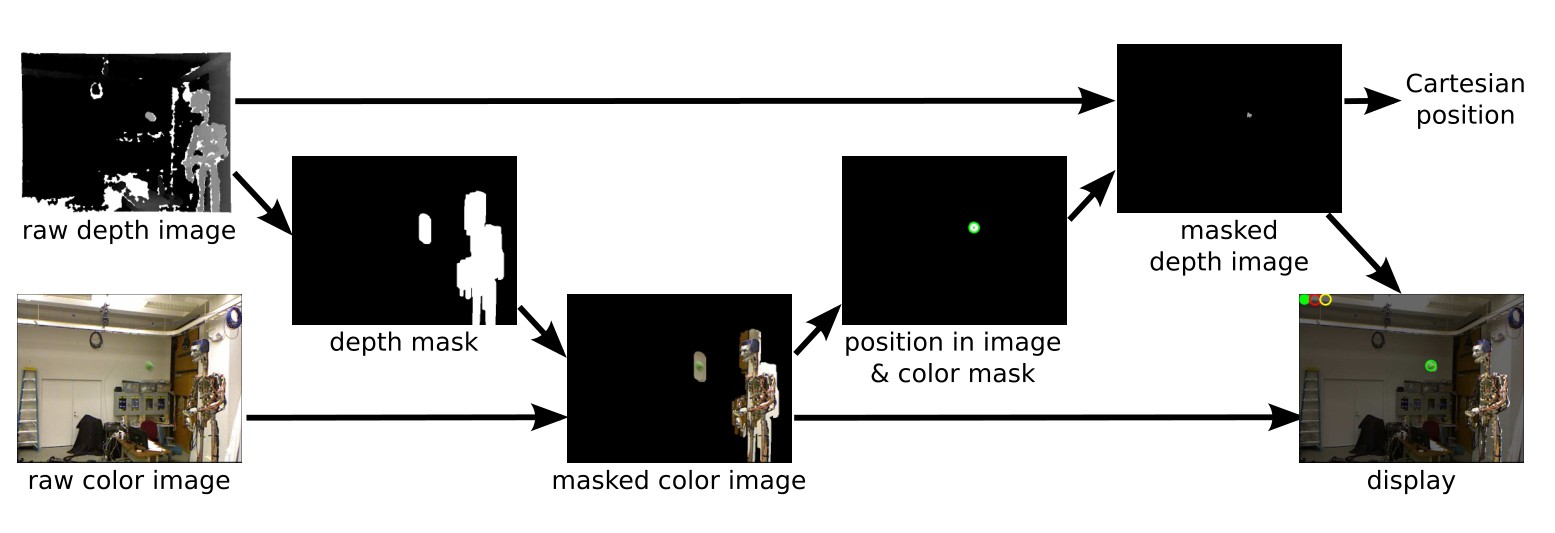
\includegraphics[scale=0.31]{img/koberpipeline.jpg}
    \caption{Bildverarbeitungs-Pipeline im Paper. ({\em Bildquelle: Playing Catch and Juggling with a Humanoid Robot\cite{kober}})}
    \label{koberpipeline}
\end{figure}

Die gelöste Aufgabe in dieser Arbeit ist also von der Grundidee her also eine ganz
ähnliche, weshalb wir den Grundaufbau der Verarbeitungsschritte auch in unserem
Vorgehen übernehmen wollten. Wie wir im Laufe der Programmierung aber feststellten,
hatte die Arbeit einige Rahmenbedingungen anders gesetzt, so dass wir auf Probleme
stießen, die sich in der Arbeit mit dem Roboter offensichtlich nicht so deutlich
gezeigt haben.

Hierbei ist zuerst zu nennen, dass die betrachteten Bälle bei uns sehr viel kleiner
waren, da wir einen tatsächlich jonglierenden Menschen betrachtet haben. In der
Arbeit mit dem Roboter wurden größere Bälle verwendet, und zu einer Zeit befindet
sich größtenteils immer nur ein Ball in der Luft.

Da in diesem Projekt die Bälle von einer Person dem Roboter zugeworfen werden,
ergeben sich auch längere Wurfbahnen und eine längere Flugzeit pro Ball. Wie
später in der Arbeit zu sehen sein wird, ist das normale Jongliermuster mit zwei
Händen teilweise so klein, dass es schwer wird, dicht aneinander vorbei fliegende
Bälle voneinander zu unterscheiden.

Zusätzlich wurde in der Arbeit mit dem Roboter auf verschiedenfarbige Bälle
zugegriffen, um diese voneinander zu unterscheiden. Dies ist eine Rahmenbedingung,
die wir so nicht wählen wollten, da die RGB-Werte, die die Kinect liefert, sehr stark
von den Beleuchtungsbedingungen abhängen und bei den verwischten Objekten, wie
wir sie in den Kinect-Aufnahmen sehen, keine robuste Erkennung möglich ist.


\subsection{Lösungsidee}

Als erste Lösungsidee haben wir in Anlehnung an die betrachtete Arbeit mit dem
jonglierenden Roboter eine eigene Zusammenstellung von durchzuführenden Bildverarbeitungsschritten
erarbeitet wie in Abbildung \ref{ourpipeline} zu sehen.

Die Verarbeitung wird auf den Einzelbildern durchgeführt, die Ergebnisse der
einzelnen Bilder werden dann kombiniert.

\begin{enumerate}
\item Auf den Tiefendaten werden ab einem bestimmten Tiefenwert (\textit{threshold})
	alle Tiefeninformationen abgeschnitten. Jongleur und fliegende Jonglierbälle sind
	somit freigestellt.
\item Auf den reduzierten Tiefendaten werden nun lokale Maxima bestimmt, welche die
	Jonglierbälle sein müssen, da sie sich näher an der Kinect befinden als der
	Jongleur. Hier sind auch die Hände enthalten.
\item Die gefundenen Maxima sind mögliche Kandidaten für tatsächlich erkannte
	Jonglierbälle.
\item Die entsprechenden Regionen werden als Maske für die RGB Daten verwendet.
\item In den interessanten Regionen der RGB Daten wird eine Erkennung für runde
	Objekte durchgeführt. Dies wird mit einer \textit{Hough Transformation} gelöst.
\item Die nun erkannten Bälle werden aufgeteilt und den einzelnen Bällen zugeordnet.
\item Für jeden Ball liegt nun also eine Reihe von Positionen vor. Um zu einer
	flüssigen Flugbewegung zu gelangen wird die Flugbahn jedes Balls mit Hilfe eines
	\textit{Kalman-Filters} modelliert und laufend aktualisiert. Mit dieser stetigen
	Positionsinformation kann die Position eines Balles also programmseitig jederzeit
	abgefragt werden.
\end{enumerate}

\begin{figure}[H]
    \centering
    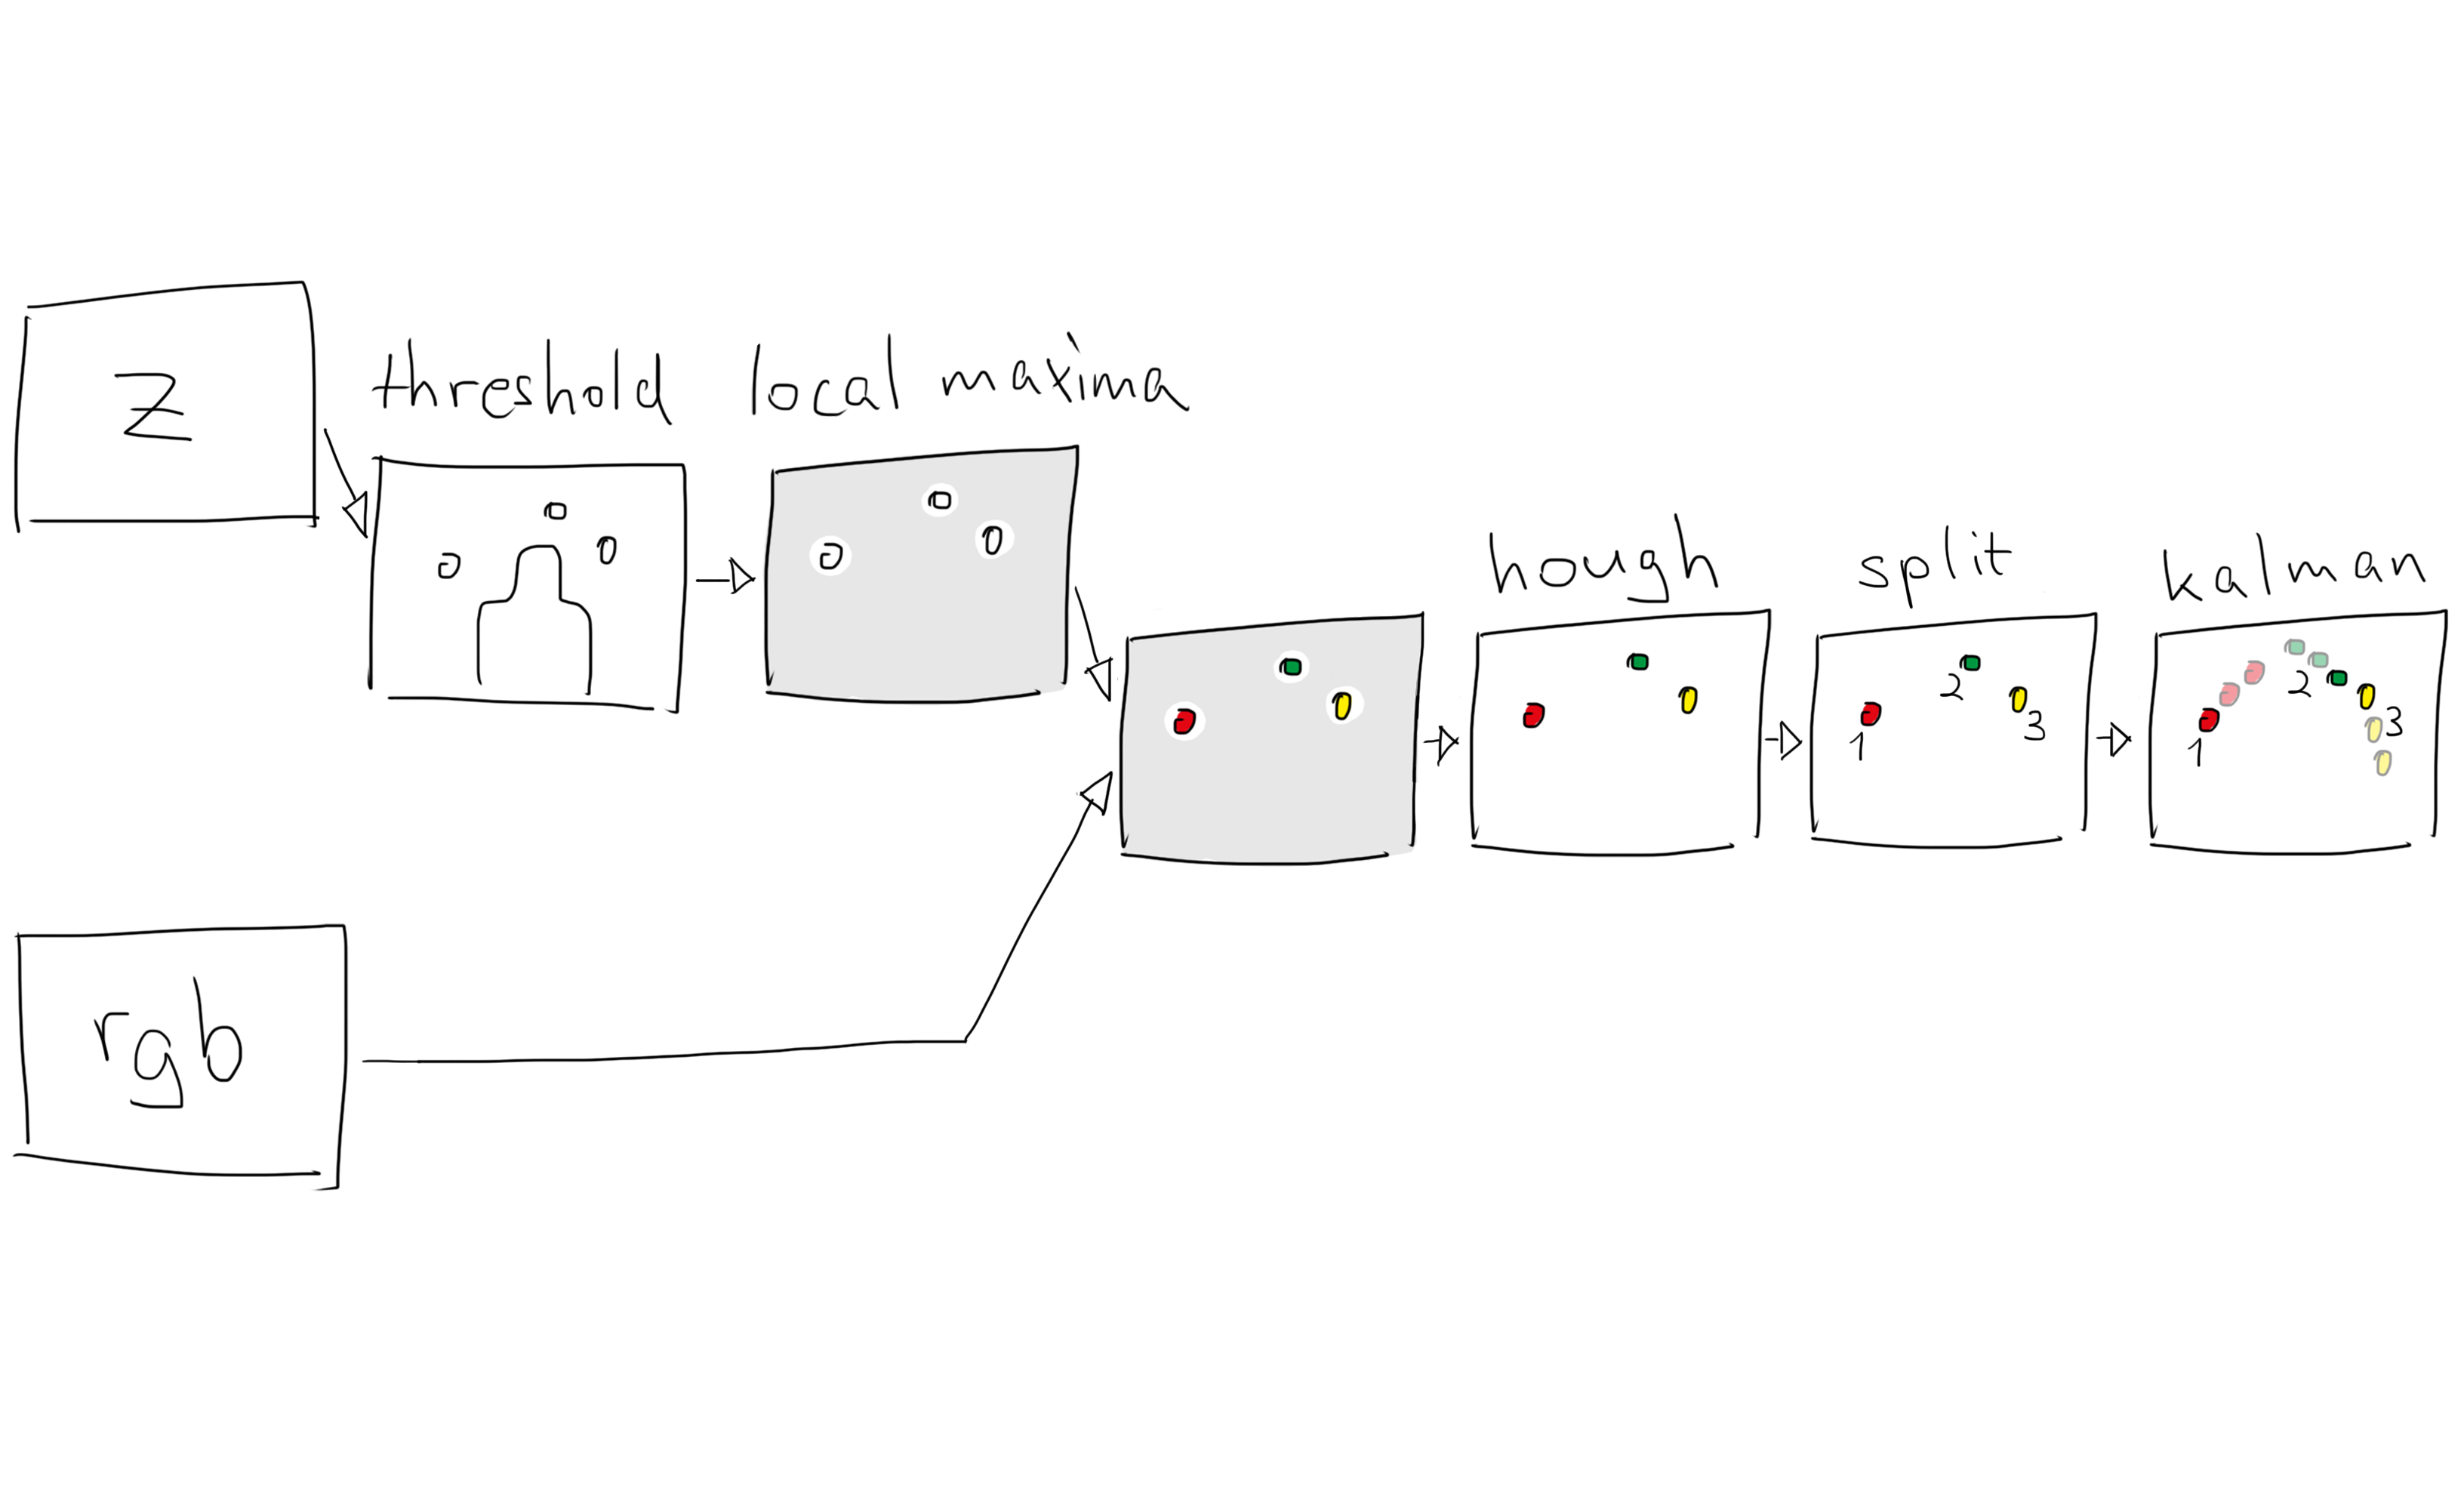
\includegraphics[scale=0.14]{img/processing-pipeline.png}
    \caption{Unsere Bildverarbeitungs-Pipeline im ersten Entwurf.}
    \label{ourpipeline}
\end{figure}

Wie sich im Laufe des Projektes heraus gestellt hat, ist diese Vorstellung der Arbeit
auf den Echtzeitdaten in einigen Schritten zu idealisiert und in anderen unnötig
kompliziert. Hierauf werden wir im finalen Schritt der Umsetzung eingehen.

\section{Finale Umsetzung}
\label{sec:final}

Im Folgenden stellen wir die finale Lösung vor, welche das Endergebnis des
Projektes darstellt. Die zahlreichen Ansätze, die wir währenddessen verfolgt haben, um zu
diesem Punkt zu gelangen, stellen wir im hieran anschießenden Kapitel vor (siehe \ref{sec:ansaetze}).

\subsection{Programmstruktur}

Das Programm besteht im Kern aus einer Schleife, in der die folgenden vier Schritte  wiederholt werden:
\begin{enumerate}
  \item Benutzereingabe verarbeiten
  \item Aktuelle Bilddaten abfragen (Von einer angeschlossenen Kinect oder aufgezeichneten Demodaten)
  \item Bilddaten verarbeiten
  \item Verarbeitete Bilddaten anzeigen
\end{enumerate}

Beim Starten des Programms über die Konsole wird zunächst die Kinect initialisiert.
Im Normalfall ist eine Kinect angeschlossen, welche dann mit Hilfe der freenect {\color{red}FIXME: cite} Bibliothek angesteuert wird. Diese liefert dann die Bild- und Tiefendaten der Kinect Kamera bzw. des Tiefensensors. Wenn keine reale Kinect zur Verfügung steht, kann alternativ auch eine Dummy-Kinect-Instanz die RGB- und Tiefenbilder bereitstellen. In diesem Fall werden zuvor aufgenommene Bildsequenzen in einer Schleife zurückgegeben um so den Datenfluss einer echten Kinect zu simulieren.
Im Anschluss daran werden sämtliche Filter initialisiert, die in der Verarbeitungsphase zum Einsatz kommen sollen.

Welche Filter aktiviert und ob eine reale Kinect verwendet oder stattdessen simuliert werden soll, kann beim Programmaufruf über die Konsole festgelegt werden. Dazu wird eine beliebige Anzahl an Parametern an das Programm übergeben. So gehört zu jedem Filter ein entsprechender Kommandozeilen-Parameter, durch den der Filter aktiviert werden kann. {\color{red}FIXME: Auflistung / Referenz der Parameter?} Dies ermöglicht es, verschiedene Filter je nach Bedarf miteinander zu kombinieren. Gleichzeitig können leicht auch nachträglich noch neue Filter hinzugefügt werden. Zudem gibt es Parameter um die Kinect zu simulieren oder Daten von einer echten Kinect aufzunehmen um diese zu einem späteren Zeitpunkt von der simulierten Kinect wiedegeben lassen zu können. Die Reihenfolge der Parameter hat hierbei keine Bedeutung und wirkt sich nicht auf die Ausführungsreihenfolge der Filter aus.

Der Aufruf für die optimale Filterkombination unseres Endergebnisses erfolgt durch \lstinline{python main.py --detectball --cutoff  --dummymode --handtracking --simplehand}

\begin{tabular}{llp{8cm}}
Parameter & Aktivierter Filter & Erklärung \\ \hline
{\lstinline!--dummymode!} & - & Verwendung von Testdaten statt einer angeschlossenen Kinect \\
{\lstinline!--cutoff!} & {\lstinline!CutOffFilter!} & Tiefenbild an Hand eines festen Schwellwertes binarisieren \\
{\lstinline!--detectball!} & {\lstinline!RectsFilter!} & Vorverarbeitung für die Ballerkennung: Regionen im Tiefenbild segmentieren \\
{\lstinline!--handtracking!} & {\lstinline!HandTrackingFilter!} & Erkennen der Hände vor der Ballerkennung \\
{\lstinline!--simplehand!} & {\lstinline!SimpleHandBallFilter!} & Ballerkennung mit simpler Zuordnung von Bällen zu Ballpositionen
\end{tabular}

{\color{red}FIXME: Verweis auf Erklärung aller möglichen Parameter}

Nach der Initialisierungsphase beginnt die oben angesprochene Programmschleife.
In jedem Schleifendurchlauf wird zunächst auf Benutzereingaben reagiert.
Ein simples Abfragen aktueller Tasteneingebaben ermöglicht es dem Benutzer einen Screenshot des momentanen RGB- und Tiefenbild zu erzeugen (Leertaste) oder das Programm zu pausieren (p) oder ganz zu beenden (beliebige andere Taste).

Im nächsten Schritt wird nun entweder von einer realen oder simulierten Kinect ein RGB- und ein Tiefenbild abgefragt. Zudem wird eine leere Liste erzeugt, in der später die Ballpositionen gespeichert werden.

Das Herz und gleichzeitig komplexeste Teil der Anwendung ist die Verarbeitung der Bilddaten.
Hierzu werden der Reihe nach sämtliche aktiven Filter auf das RGB- und Tiefenbild sowie die Ballpositionen angewandt.

Dazu verfügt jeder Filter nun über eine \lstinline{filter} Methode mit drei zwingenden und einem optionalen
Parameter. Der optionale Parameter \lstinline{args} ist ein Dictionary und wird lediglich für das Ablegen von
Meta-Informationen verwendet, wie etwa Zusatzinfos zur Visualisierung.

Als Ergebnis von jedem Filter wird analog zum Filteraufruf ein Drei-Tupel zurückgegeben, bestehend aus RGB- und Tiefenbild sowie der Liste von Ballpositionen. Die so erhaltenen Daten dienen wiederum dem nächsten Filter als Eingabe-Parameter. Somit können die Filter nach und nach die Rohdaten manipulieren und verarbeiten.

Ein minimaler Filter ohne Funktionalität sieht demnach wie folgt aus.

\begin{lstlisting}[language=Python,caption={Grundstruktur eines Filters. In diesem Beispiel werden die Eingabedaten unverändert zurückgegeben.}]
class DummyFilter(object):

    def filter(self, rgb, depth, balls, args = {}):

        # ...

        return rgb, depth, balls
\end{lstlisting}

Zur besseren Übersicht über die Vielzahl der Filter haben wir diese für die finale Umsetzung in Packages organisiert. Jeder Filter liegt dabei in einem eigenen Modul vor (genauso wie jede der Ballerkennungsmethoden, auf die wir später zu sprechen kommen. Die Strukturierung in vier Packages je nach Aufgabe der einzelnen Komponenten erlaubt eine übersichtliche Codebasis und selbsterklärende \lstinline{import} Statements.

\begin{tabular}{ll}
\textbf{Package} & \textbf{Inhalt} \vspace{0.1cm} \\
{\lstinline!src.kinect!} & Module zum Ansprechen der Kinect und für Demodaten \\
{\lstinline!src.preprocessing!} & Filter der Datenvorverarbeitung\\
{\lstinline!src.balldetection!} & Hand- und Ballerkennung\\
{\lstinline!src.visual!} & Visualisierung und finale Ausgabe der Daten\\
{\lstinline!src.application!} & Beispielhafte Anwendungen auf Basis unseres Projekts
\end{tabular}

Nachdem alle Filter ausgeführt wurden, werden die resultierenden Bilder angezeigt. Beim Programmstart kann hierbei auch wieder über einen Parameter festgelegt werden, ob entweder das RGB- oder das Tiefenbild angezeigt werden soll. Damit ist ein Schleifendurchlauf beendet und der nächste Durchgang beginnt mit dem laden der nächsten Bilddaten.

\subsection{Programmfluss}

Die Verarbeitung der Bilddaten durch die Filter lässt sich in mehrere Bereiche unterteilen.
Zunächst werden die Rohdaten vorverarbeitet um anschließend nur noch mit normalisierten
Tiefeninformationen zu arbeiten. Im nächsten Schritt werden mögliche Ballpositionen bestimmt.
Diese werden nun genutzt, um die Ballpositionen zeitlich einem Ballverlauf zuzuordnen, der von einzelnen Tiefenbildern abstrahiert und eine Ballbewegung über mehrere zeitlich aufeinander folgende Bilddaten hinweg beschreibt.
Im letzten Schritt werden dann aus den Ballverläufen mehrere bereinigte Wurfparabeln erzeugt.
Die einzelnen Arbeitsschritte werden im folgenden noch detailierter betrachtet.

\subsubsection{Schritt 1: Tiefendaten vorverarbeiten}\label{sec:preprocess}

Die Kinect liefert Tiefenwerte im Bereich von 0 bis 2047, wobei ein höherer Wert
einen größeren Abstand bedeutet. Die 0 steht hierbei für einen Pixel, in dem keine
Tiefeninformation vorliegt.

Für unsere Aufgabe ist Beschaffenheit des Hintergrundes irrelevant. Außerdem nehmen
wir einen isoliert stehenden Jongleur an. Zwischen der Tiefenebene des Jongleurs
und dem Sensor befinden sich laut unsere Annahme keine Objekte außer den
Jonglierbällen. Ein erster Schritt besteht daher im Binarisieren der Tiefendaten.
Ab einem festen Abstand zur Kinect werden alle weiter entfernt liegenden Werte auf 0
(=schwarz) gesetzt. Alle näher am Sensor befindlichen Punkte werden auf 2047 (=weiß)
gesetzt. Der Schwellwert, an dem diese Binarisierung getroffen wird, ist von uns
zuerst auf 2100 gesetzt worden, da dies in den von uns aufgezeichneten Testdaten
genau einer Grenze direkt vor dem Körper des Jongleur entsprach, so dass wir
die Bälle und Hände des Jongleurs isoliert hatten. Im weiteren Verlauf haben wir mit
einer dynamischen Bestimmung dieser Grenze experimentiert, letzten Endes dann aber
doch diesen festen Wert belassen. Bei der tatsächlichen Anwendung in Echtzeit
positioniert man sich also an einen festgelegten Punkt im Raum. Dies ist tatsächlich
auch nicht störend. Da direktes visuelles Feedback von unserer Anwendung deutlich
macht, wann man richtig steht, ist auch keine feste Bodenmarkierung nötig.

{\color{red}FIXME: Bild Tiefendaten -> Binarisiertes Bild}

Auf Grund der Funktionsweise der Kinect mit dem RGB-Sensor und dem knapp daneben
befindlichen Infrarotsensor sind die RGB- und Tiefendaten leicht gegeneinander
verschoben. Hierbei hängt die Verschiebung vom Abstand eines Raumpunktes zur Kinect
ab (Parallaxeffekt). Zwar arbeitet unsere Analyse nur auf den gelieferten
Tiefendaten, so dass wir für die Ballerkennung diese Verschiebung ignorieren
könnten. Für die Visualisierung überlagen wir aber die gewonnene Information mit
den RGB-Daten, so dass wir hierfür diesen Fehler korrigieren müssen. Diese
Korrektur ist daher auch Teil der Vorverarbeitung. Glücklicherweise unterstützt
die \lstinline{freenect} Bibliothek in der zum Projektzeitpunkt nur als
\lstinline{unstable} erhältlichen Version diese Fehlerkorrektur von Haus aus. Nötig
ist hierzu lediglich die Angabe eines bestimmten Formats beim Anfordern eines
Frames von Tiefendaten: \lstinline{freenect.get_depth(format=4)}
Erzeugt dieser Aufruf einen Fehler, so ist dies ein Hinweis, dass nicht die korrekte
Version der \lstinline{freenect} Bibliothek verwendet wird.

Durch die Funktionsweise der Kinect, kann keine Tiefeninformationen an Flächen gewonnen werden, die orthogonal zum Sensor der Kinekt stehen, da dort kein Infrarotlicht zum Sensor reflektiert wird.
Das Tiefenbild besitzt an diesen Stellen dementsprechend keine verwendbaren Tiefenwerte. Stattdessen wird an diesen Positionen der Wert 0 eingefügt. Dies führt an den meisten Objekt-Kanten und insbesondere bei den Jonglierbällen zu einem um das Objekt liegenden Rahmen von Null-Werten. Durch das zuvor angesprochene Binarisieren, werden diese Werte dann im Zuge der Vorverarbeitung auf den maximalen Tiefenwert gesetzt. Aufgrunddessen schrumpfen die Objecte um wenige Pixel. Für die Bälle bedeutet dies, dass deren Durchmesser im Tiefenbild etwas kleiner ist, als der im RGB-Bild. Dies hat aber nur minimale Auswirkungen auf die spätere Erkennung und Bestimmung der Position der Jonglierbälle.
Das füllen dieser Löcher im Tiefenbild kann alternativ auch kontext-sensitiv ausgeführt werden. Da die momentane Behandlung jedoch zufriedenstellende Ergebnisse liefert, wurde auf einen komplexeren Algorithmus verzichtet. Dieser würde die Ballerkennung wahrscheinlich nur unwesentlich verbessern und würde somit nur unnötig Rechenzeit beanspruchen.
{\color{red}FIXME Tiefenbild eines balls vorher und nacher}

{\color{red}FIXME: häh? oben hast du das bild doch schon binarisiert? außerdem ergibt der satz keinen sinn von 256 auf irgendetwas zu reduzieren damit man nur bis 255 arbeitet?! }
Hatten wir ursprünglich noch überlegt, die Tiefenwerte von 256 bit auf einen
niedrigeren Wert zu reduzieren, um in der Verarbeitung der Einfachheit halber nur
mit Werten zwischen 0 und 255 arbeiten zu müssen, so haben wir uns dann doch gegen
diese Reduzierung entschieden. Lediglich für den Fall der Visualisierung der
Tiefendaten führen wir eine entsprechende Transformation durch, um auf Grauwerte
zwischen 0 und 255 abzubilden.

\subsubsection{Schritt 2: Regions Of Interest isolieren}
\label{sec:roi}

Um den Hintergrund zu entfernen und die Bälle freizustellen, wurden zwei Ansätze getestet:

\begin{itemize}
\item[A.]Möglichst keine Objekte in der Tiefenebene zwischen dem Spieler und der Kinect platzieren, auch nicht am Rand. Die Tiefenwerte
werden nun ab einem gewissen Wert einfach abgeschnitten, so dass in diesen im optimalen Fall nur noch die Bälle sowie die Hände des
Jongleurs verbleiben. Hier wird also die Annahme getroffen, dass der Spieler auf einer Linie oder ähnlichem in einem festen Abstand zur
Kinect steht. Die Tiefendaten werden nun noch binarisiert.
\item[B.]Mit einem temporalen Filter sich bewegende Regionen isolieren. Dieses erlaubt auch störende Objekte wie Stühle am Rand sowie
einen flexiblen Abstand des Spielers zur Kinect. Nach einer Implementierung wurde aber deutlich, dass das Verfahren bei schnellen Bewegungen
(wie dem Ballwurf) nicht zuverlässig ist. Außerdem traten vermehrt Probleme mit unscharfen Objekträndern und Rauschen auf, die aber mit Funktionen der VIGRA\cite{vigra} kompensiert werden konnten. Die Probleme mit schnellen Bewegungen verblieben aber und es kamen noch technische Hürden hinzu, wie die VIGRA\cite{vigra} als weitere Abhängigkeit.
\end{itemize}

Wir stellten fest, dass Ansatz A völlig ausreichend für unsere Zwecke ist. Die Einschränkung der Spielerposition ist ebenfalls nicht störend, da dies sogar interaktiv durchgeführt werden kann (so lange nach vorne gehen, bis das System vernünftige Werte liefert - kein aufwändiges Abmessen nötig). Weiterhin redgt dies sogar den Spieler an, seine Ballwürfe kontrolliert durchzuführen, ohne dass diese ihn zu Positionsveränderungen zwingen.

\subsubsection{Schritt 3: Bälle in Frame-Folgen einander zuordnen}

Bevor potentielle Ballpositionen konkreten Ball-Instanzen zugeordnet werden, findet eine kurze Vorverarbeitung statt, bei der Regionen im binarisierten Ergebnis des vorherigen Schrittes als Rechtecke umzeichnet werden, wofür einfach die OpenCV-Funktion \lstinline{cv.BoundingRect} verwendet wird, die genau diese Aufgabe erfüllt.
Kleine Rechtecke und solche, die den Bildrahmen berühren, werden hierbei bereits herausgefiltert.

Durch die resultierende Liste von Rechtecken wird iteriert und jeder
Rechteckmittelpunkt als mögliche Ballposition aufgefasst (die kürzere Rechteckskante
wird als Balldurchmesser gespeichert, vorerst aber ignoriert).

\vspace{0.5cm}
\begin{lstlisting}[language=Python,caption={RectsFilter.py, Ausschnitt}]
# ...

        storage = cv.CreateMemStorage(0)
        contour = cv.FindContours(depth_cv, storage, cv.CV_RETR_CCOMP, cv.CV_CHAIN_APPROX_SIMPLE)
        points = []

        ball_list = [] # collect ballpositions in loop
        while contour:
            x,y,w,h = cv.BoundingRect(list(contour))
            contour = contour.h_next()

            # filter out small and border touching rectangles
            t = 2 # tolerance threshold
            minsize = 5
            if x > t and y > t and x+w < self.WIDTH - t and y+h < self.HEIGHT - t and w > minsize and h > minsize:
                x -= 5
                y -= 5
                w += 10
                h += 10
                x, y = self._nullify(x), self._nullify(y) # why is this necessary now?

                ball_center = (x+w/2, y+h/2)
                ball_radius = min(w/2, h/2)
                ball_list.append(dict(position=ball_center, radius=ball_radius))

                # Draw rectancle with info
                cv.PutText(rgb_cv, '%d/%d' % (x, y), (x,y-2) , self.font, (0, 255, 0))
                cv.Rectangle(rgb_cv, (x, y), (x+w, y+h), cv.CV_RGB(0, 255,0), 2)

        args['balls'].addPositions(ball_list)
\end{lstlisting}

Es liegt nun
für jeden Frame eine Liste von möglichen Ballpositionen vor. Diese setzen sich aus tatsächlichen Ballpositionen, Positionen in denen sich die Hände befinden sowie potentiell weiteren Hindernissen im Sichtfeld der Kinect zusammen, wobei wir diese in unseren Testdaten vermieden haben. Bei den tatsächlichen Ballpositionen ist zu beachten, dass diese etwas ungenau sind und mit mehreren Pixeln vom tatsächlichen Ballmittelpunkt abweichen können.

\begin{figure}[H]
    \centering
    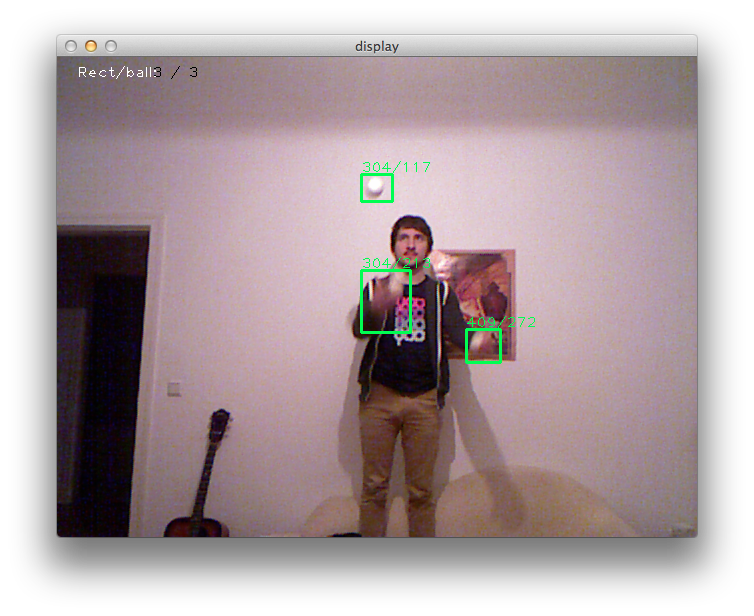
\includegraphics[scale=0.5]{img/rects-1.png}
    \vspace{-0.5cm}
    \caption{FIXME}
    \label{rects-1}
\end{figure}

\begin{figure}[H]
    \centering
    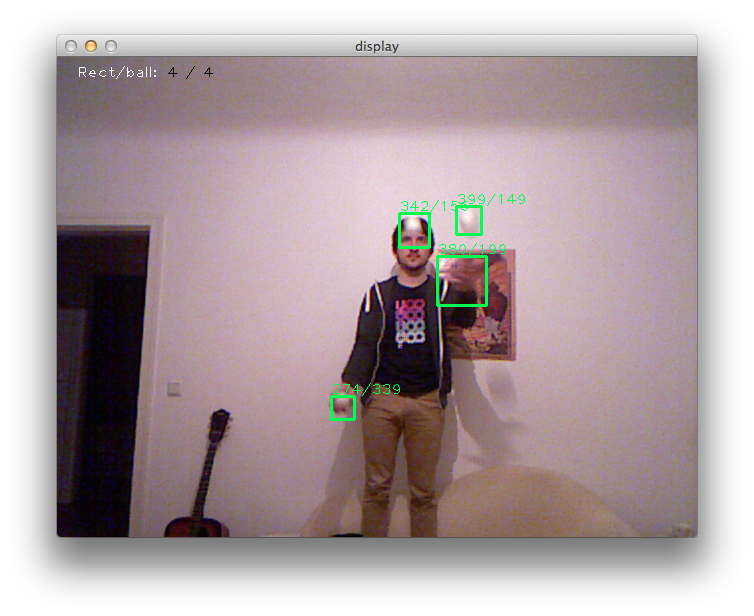
\includegraphics[scale=0.5]{img/rects-2.png}
    \vspace{-0.5cm}
    \caption{FIXME}
    \label{rects-2}
\end{figure}

\begin{figure}[H]
    \centering
    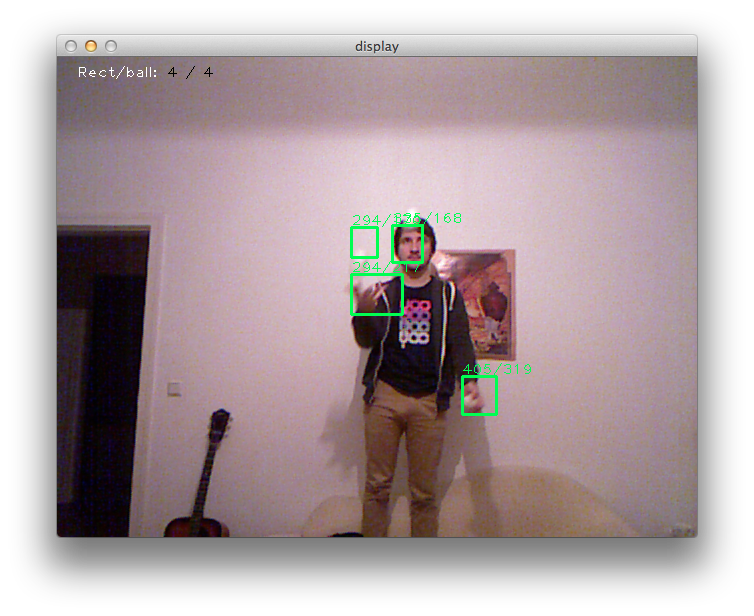
\includegraphics[scale=0.5]{img/rects-3.png}
    \vspace{-0.5cm}
    \caption{FIXME}
    \label{rects-3}
\end{figure}

\begin{figure}[H]
    \centering
    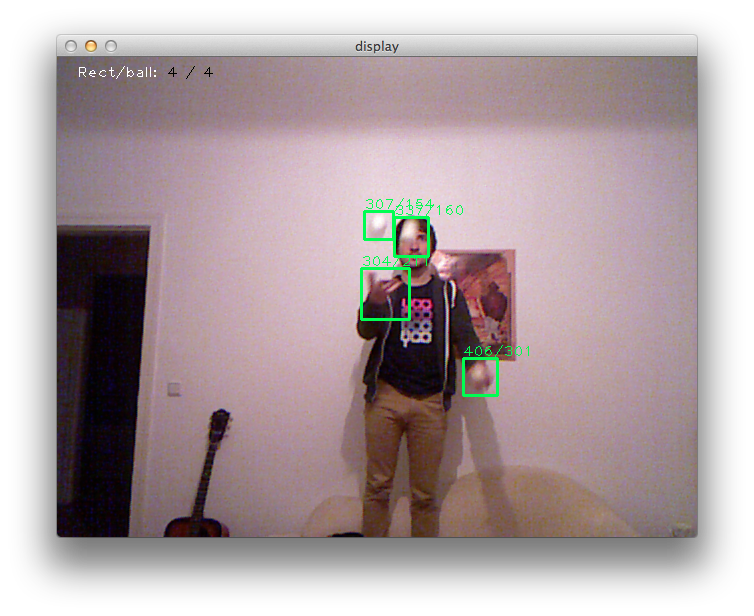
\includegraphics[scale=0.5]{img/rects-4.png}
    \vspace{-0.5cm}
    \caption{FIXME}
    \label{rects-4}
\end{figure}

Im Folgenden kommt die Hauptaufgabe dieses Schritts: Das Zuordnen der potentiellen
Punkte zu tatsächlichen Ballinstanzen, wobei diese Zuordnung über mehrere Frames
hinweg eine neue Position einem bestehenden Ball zuordnen soll.

Dies ist, wie es sich herausgestellt hat, der aufwändigste Schritt - zumindest der, mit dessen Lösung wir die meiste Zeit verbracht haben. Mehr dazu im später folgenden Abschnitt zu den von uns ausprobierten Ansätzen \ref{sec:ansaetze}.

Unsere endgültige Version der Ballerkennung ist in \lstinline{SimpleHandBallFilter} 
implementiert. Robust funktioniert dieser Filter nur, wenn vorher der Filter 
\lstinline{HandTrackingFilter} angewandt wurde. \lstinline{HandTrackingFilter}  betrachtet die gefundenen potentiellen Ballpositionen und identifiziert die beiden Hände des Jongleurs. Die als Hände identifizierten Positionen werden aus der Liste entfernt, so dass \lstinline{SimpleHandBallFilter} im Folgenden auf den übrig gebliebenen Positionen arbeitet. Hierzu kann sehr viel zuverlässiger bestimmt werden, welche Position tatsächlich ein fliegender Ball ist. Bälle, die sich momentan in der Hand des Jongleur befinden, werden hierbei ignoriert bzw. nicht als Bälle erkannt. 

Wir wollen diese beiden Filter im Folgenden im Detail betrachten.

\lstinline{HandTrackingFilter}

Bei Initialisierung des Filters werden zwei \lstinline{Hand} Instanzen an beliebiger Initialposition erstellt.

\begin{lstlisting}
self.left = Hand((100, 100))
self.right = Hand((200, 200))
\end{lstlisting}

In einem Filteraufruf wird das übergebene \lstinline{args} Dictionary dann 
verwendet, um zu markieren, dass der Filter die Handobjekte zugeordnet hat. Es 
werden außerdem Referenzen zu den Instanzen für beide gesetzt. Diese Information ist 
vor allem für die spätere Visualisierung (optionales Einzeichnen der Handpositionen)
nötig, kann aber auch für andere Weiterverarbeitung verwendet werden.

\begin{lstlisting}
args['hands'] = True
args['hand_left'] = self.left
args['hand_right'] = self.right
\end{lstlisting}

Um die Hände in der Eingabeliste \lstinline{positions} von potentiellen Ball-
Positionen zu identifizieren, wird
die Mitte des Jongliermusters bestimmt. Dies ist der Mittelwert aller x-Koordinaten
der in der Liste befindlichen Positionen. 

\begin{lstlisting}
# determine center of juggling pattern
if len(positions) > 0:
    centerX = sum([b['position'][0] for b in positions]) / len(positions)
else:
    centerX = 320
args['centerX'] = centerX
\end{lstlisting}

Anhand dieses Mittelwertes werden die Positionen aufgeteilt in alle Positionen 
rechts und alle Positionen links von diesem Wert. In jedem der beiden resultierenden
Liste wird dann die jeweils unterste Position als Hand identifiziert.

\begin{lstlisting}
# two properties for match each hand (left & right)
handProps = [(self.left, lambda p: p['position'][0] <= centerX),
    (self.right, lambda p: p['position'][0] > centerX)]

for hand, filterKey in handProps:
    # filter in right and left positions
    filtered = filter(filterKey, positions)
    if len(filtered) > 0:
        lowest = sorted(filtered, key=lambda p: -1*p['position'][1])[0]
        lowestPosition = lowest['position']

        hand.update(lowestPosition)
        positions.remove(lowest)
\end{lstlisting}

Entscheidend ist das das abschließende Entfernen der identifizierten Hand aus der 
Liste \lstinline{positions}. Diese Liste vom Filter zurück gegeben und im 
nachfolgenden Filter \lstinline{SimpleHandBallFilter} verwendet. Für diesen Filter
ist es dann entscheidend, dass sich in der Liste nur noch Positionen von fliegenden
Bällen befinden.


\lstinline{SimpleHandBallFilter}

Sind die Hände erkannt und aus der Positionsliste entfernt, ist dann also die 
Aufgabe des folgenden Filters, die potentiellen Ballpositionen durchzugehen und zu
versuchen, sie bereits erkannten Bällen aus dem vorherigen Frame zuzuordnen. Wird
kein passender bereits erkannter Ball erkannt, so wird an dieser Position ein 
neuer Ball initialisiert. Entsprechend werden Bälle aus dem vergangenen Frame, für
die keine passende Folgeposition gefunden wurde, aus der Liste der aktuell 
vorhandenen Bälle entfernt.

{\color{red} FIXME Flo: Filter erklären}




\subsubsection{Schritt 4: Bereinigte Wurfparabel}

Das fehlt uns noch. Aber aus den gelieferten Daten wollen wir dann höher-levelige Informationen abstrahieren. Objektanzahl, Wurfhöhen, Würfe zählen, etc.




\section{Ansätze im Laufe des Projektes}
\label{sec:ansaetze}

Im Folgenden beschreiben wir die Arbeitsschritte, wie wir sie an Hand unserer
Grundplanung ausgeführt haben. Wir gehen dabei auf die Schwierigkeiten ein, auf die
wir getroffen sind, wodurch dann deutlich wird, weshalb wir zu unserer endgültigen
Umsetzung gekommen sind. Diese finale Umsetzung haben wir im Abschnitt \ref{sec:final} beschrieben.

\subsection{Anfängliche Programmstruktur}

Die ersten Tests, die wir mit der Kinect und bildverarbeitenden Verfahren
ausprobiert haben, bestanden aus wenigen Schritten und wurden in einer
simplen Schleife gelöst, die bei Druck der ESC Taste verlassen wurde. Zu Beginn
eines Schleifendurchlaufes wird ein neuer RGB Frame und die zugehörigen
Tiefendaten geholt. Danach folgt schrittweise Verarbeitung dieser Daten je nach
gewünschtem Zweck.


\begin{lstlisting}[language=Python, caption={Jeder Schleifendurchlauf entspricht einem Frame. Mit der SPACE Taste wird der aktuelle Frame als Bild gespeichert, jede andere Taste beendet die Schleife und somit das Programm.}]
    def loop(self):
        """ Start the loop which is terminated by hitting a random key. """
        while self.running:
            if self.record:
                self.snapshot()
            else:
                self._step()
            key = cv.WaitKey(5)
            self.running = key in (-1, 32)
            if key == 32: # space bar
                self.snapshot()

    def _step(self):
        """ One step of the loop, do not call on its own. Please. """
        # Get a fresh frame
        (rgb, depth) = self.kinect.get_frame()

        # ... normalize values

        # ... processing

        # transform to open CV representation
        rgb_opencv = cv.fromarray(np.array(rgb[:,:,::-1]))

        # Display image
        cv.ShowImage('display', rgb_opencv)

\end{lstlisting}



Nun möchten wir je nach betrachtetem Arbeitsschritt aber verschiedene
Verarbeitungsstufen ausführen oder ausklammern, so dass wir irgendwie eine
Parametrisierung finden mussten. Wir haben uns für ein Konzept von Filtern
entschieden, wobei zu Programmstart eine Liste mit gewünschten Filtern erstellt
wird und diese in der Hauptschleife nacheinander ausgeführt werden (die Originaldaten
werden also in den ersten Filter gegeben, das Ergebnis dieses Filters wird als
Eingabe für den zweiten Filter verwendet und das Ergebnis des letzten Filters
in der Liste wird dann als Gesamtausgabe visuell dargestellt.

Die RGB- und Tiefendaten werden vom freenect Modul als numpy Arrays zurückgegeben.
Die Ausgabe erfolgt über ein von OpenCV erzeugtes Fenster, welches Daten für
OpenCV erwartet. Die numpy Arrays müssen also an einer Stelle umgewandelt werden.
Zusätzlich haben wir schnell festgestellt, dass einige gewünschte Operationen
entweder nur in numpy oder nur in OpenCV zur Verfügung stehen. Ein mehrfaches
Umwandeln von einem Format in das jeweils andere ist aus Performanz-Gründen
natürlich zu vermeiden. Um in der Entwicklung nicht immer darauf achten zu müssen,
welcher Filter welche Eingabe erwartet und welche Ausgabe liefert, haben wir uns dazu
entschieden, jeden Filter als Eingabe Daten in numpy Darstellung zu liefern und auch
für die Ausgabe numpy zu erwarten. Dies erlaubt uns eine von außen identische
Betrachtung der Filter, auch wenn einige Filter intern eine Umwandlung durchführen
müssen. Bei etwaigen Problemen wollten wir die Performanz unserer Lösung getrennt
betrachten, um zu Beginn lediglich über eine funktionierende Lösung nachdenken
zu müssen.

Waren die Filter ursprünglich als isolierte Einheiten mit simplem
Input-Output-Verhalten von Bild- bzw. Tiefendaten gedacht, fiel uns schnell auf,
dass einige Filter Zusatzinformationen liefern, die von anderen Filtern gebraucht
werden. Um Filter nicht intern Unteraufrufe von anderen Filtern oder Komponenten
ausführen zu lassen (dies wäre ebenfalls eine denkbare Lösung), entschieden wir uns
für ein Objekt, das von der Hauptkomponente des Programms in jeden Filter
hineingereicht wird und in dem jeder Filter Informationen ablegen und abfragen kann.
Natürlich ist dies abhängig von der Reihenfolge der Filter und einige Filter haben
als implizite Vorbedingung, dass andere Filter bereits ausgeführt wurden, dies haben
wir der Einfachheit halber aber nicht expliziert formuliert, im Zweifelsfall wird
beim ersten Ausführen einer nicht korrekten Filterkombination oder -reihenfolge ein
Laufzeitfehler geworfen, da Informationen in dem übergebenen Objekt noch nicht
vorhanden sind. Dieses Objekt ist ein schlichtes Python dictionary.


{\color{red} FIXME: Diagramm Programmstruktur (so cool skizziert, nicht ganz formell UML)}

{\color{red} FIXME: bisschen Python Listing um diese Filter-Konzepte und das args dictionary zu zeigen}

Genau diese Problematik, dass die Abhängigkeiten von Filtern nur implizit festgelegt
ist und zur Laufzeit Fehler auftreten, weil eine benötigte Information im
\lstinline{args} dictionary nicht vorhanden ist, hat uns aber noch nicht zufrieden
gestellt. Daher haben wir das Filterkonzept weiter angepasst.

FIXME: Pointer finale Umsetzung

\subsection{Weitere Ansätze und Bildverarbeitungsverfahren}

\subsubsection{Temporale Ballerkennung}
\label{sec:temporal}

Ein alternativer Ansatz beruht auf der Idee, sämtliche sich nicht bewegende Teile im Tiefenbild herauszufiltern. Motiviert ist dies, um Teile der Vorerarbeitung des Tiefenbildes und der Ballerkennung flexibler zu gestalten. Bei der Vorverarbeitung wird, wie in \ref{sec:preprocess} beschrieben, davon ausgegangen, dass sich der Jongleur in einem bestimmten Abstand zum Kinect-Sensor befindet und seine Hände  die Bälle in einer bestimmte Distanz zu seinem Körper jonglieren. Zudem dürfen keine anderen Objekte,
beispielsweise Stühle, in der gleichen Ebene stehen und von der Kinect erfasst werden.
Der Temporale Filter entstand mit dem Wunsch, diese Einschränkung aufzuweichen und nach Möglichkeit komplett zu eliminieren.

Grundgedanke beim Temporalen Filter ist das Vergleichen von zwei zeitlich nah beieinanderliegenden Tiefenbildern.
Nur dort, wo sich Objekte in dem Zeitfenster zwischen den Aufnahmezeitpunkten der Tiefenbilder bewegt haben,
unterscheiden sich die Tiefendaten. Betrachtet man nur die Unterschiede, werden ausschließlich bewegte Objekte gefunden und sämtliche starre Objekte werden automatisch nicht mehr erfasst.
Zudem geschieht dies unabhängig von der Entfernung der Objekte zum Sensor.

Dabei gilt es aber zu bedenken, dass das Rauschen in den Tiefenbildern zu einem verrauschten Differenz-Bild führt. Zudem bewegt sich auch der Körper des Jongleurs leicht beim jonglieren. Das Verfahren hierbei muss also geeignete Maßnahmen implementieren, die diese Störeinflüsse kompensieren.

Da dieser Ansatz verschiedene Tiefenbilder miteinander vergleicht, muss dem Filter Zugriff auf Daten aus der Vergangenheit ermöglicht werden.
Zu diesem Zweck sammelt der Filter die Tiefenbilder intern in einem Buffer.
Nachdem zum ersten mal ein Bild im Buffer gespeichert wurde, kann im nächsten Filterdurchgang das momentane Tiefenbild mit dem vorherigen verglichen werden.
Bei der Implementation des Filters wird hierbei ein Differenzbild in Form eines Binärbildes erzeugt.
Für jeden Pixel wird überprüft, ob der Tiefenwert im alten Tiefenbild größer ist, als der entsprechende Pixel im aktuellen Tiefenbild.
Jenachdem wird entweder eine 1 oder eine 0 im Binärbild gespeichert.
Da bei dieser Betrachtung jeder Pixel unabhängig von den Werten in seiner unmittelbaren Umgebung verarbeitet wird, macht sich hierbei etwaiges Rauschen in den Tiefendaten besonders bemerkbar.
{\color{red}FIXME Verrauschtes Tiefen-Differenzbild}
Um diese Fehlerhaften Pixel zu entfernen und falsch positive Ballpositionen zu verhindern, wird das Binärbild zunächst durch Erosion und anschließende Dilatation geglättet.
Die Bälle im Tiefenbild sind großflächig genug, so dass sie von diesem Vorgang nur bedingt beeinflusst werden.
Die Chance, durch die Erosion einen Ball komplett zu löschen ist daher nur sehr gering.
Im Gegensatz dazu verschwindet ein Großteil der verrauschten Pixel.
Diese bilden selten zusammenhängende Flächen und wenn, dann sind diese nur wenige Pixel groß.
{\color{red}FIXME Tiefen-Differenzbild nach Erosion + Dilatation}
Als Nebeneffekt werden hierbei auch einige Bereiche geglättet, in denen Körperbewegungen zu einer temporalen Veränderung im Tiefenbild geführt haben. Da sich der Körper im Vergleich zu den fliegenden Bällen nur mit einer sehr geringen Geschwindigkeit bewegt, entstehen hier auch nur schmalere Bewegungsschatten im Binärbild.
Nach dieser ersten Glättung des Differenzbildes, werden zusammenhängende Bereiche extrahiert.
Unter der Annahme, dass die Bälle im Binärbild eine Fläche bilden, die eine Mindestanzahl an Pixeln nicht unterschreitet, findet anschließend eine erneute Überprüfung statt. Alle zusammenhängende Bereiche, die in der Summe zu wenig Pixel haben, werden ignoriert.
Nur die Bereiche, die groß genug sind, werden gesammelt und als potientelle Bälle in einer Liste gespeichert.
Diese Liste wird anschließend in der Filterkette weitergerreicht und bildet somit das Ergebnis des temporalen Ballerkennnugsfilters.
{\color{red}FIXME Ballpositionen}

Große Auswirkung auf die Güte der Ballpositionen hat hierbei der zeitliche Abstand der beiden Tiefenbilder, die zu Beginn verglichen werden. Wenn die Bilder zeitlich so nah beieinander liegen, dass sich die Ballflächen in den beiden Frames teilweise überschneiden, entstehen halbmondförmige Flächen im Binärbild.
Diese werden dann aber unter Umständen von dem Erosions-Prozess vernichtet.
Oder aber in der Pixelsumme so stark reduziert, dass sie in der anschließenden Überprüfung aussortiert werden.
Gleiches kann auch im Scheitepunkt der Wurfparabel auftreten. Auch bei größeren zeitlichen Abständen besitzen die Bälle an dieser Stelle eine zu geringe vertikale Geschwindigkeit um sich in aufeinander folgenden Bildern nicht zu überschneiden.
{\color{red}FIXME Halbmonde}
Auf der anderen Seite führt ein zeitlich zu großer Abstand zwischen den zwei Tiefenbildern dazu, dass auch langsame Bewegungen des Jongleurs zu großen Bewegungsschatten führen, die im Folgenden nicht mehr herausgefiltert werden können.

Zur Erosion, Dilatation und zum Finden von zusammenhängenden Bereichen im Binärbild kam hierbei die Bildbearbeitungsbibliothek VIGRA {\color{red}FIXME quelle} zum Einsatz.
Dies ermöglicht eine effiziente Durchführung der entsprechenden Operationen.
Dennoch machen sich die zusätzlichen Berechnungen in der Framerate bemerkbar und erschweren die Echtzeitfähigkeit der Ballerkennung. Gepaart mit der teilweise fehlerhaften Ballerkennung,
bedingt durch die Selbst-Überdeckung der Bälle in den langsameren Teilen der Wurfbewegung, wurde dieser Ansatz letztendlich für die endgültige Lösung verworfen und dementsprechend auch nicht weiter ausgearbeitet.

\subsubsection{Kalman Filter}

{\color{red} FIXME ROLF: Schaubilder, evtl. Beispiel mit Zeichnungen oder so, Python Code Beispiel}

Der Kalman Filter ist ein in 1960 von Rudolf E. Kálmán vorgestellter Algorithmus, welcher aus mehreren ungenauen Messungen versucht, die tatsächlichen Daten, die diesen Messungen zu Grunde liegen, zu estimieren.\cite{kalman} Solche Ungenauigkeiten können durch die Messsensoren entstehen, wenn diese aus verschiedenen Gründen nicht präzise genug aufnehmen können, oder auch durch ein Rauschen der Aufnahmequelle. Mit dem Kalman-Filter können so über einen bestimmten Zeitraum aufgenommene Daten mit möglichst vielem Wissen über potentielle Messabweichungen genauer bestimmt werden, als mit nur einzelnen Messungen.

Dieser Algorithmus wird heutzutage in vielen Bereichen eingesetzt, sehr oft aber in der Navigationstechnologie von Fahrzeugen aller Art. Die Position eines Fahrzeuges wird beispielsweise über GPS empfangen. Diese Technologie kann selbst mit einer zusätzlichen Korrektur (WAAS/EGNOS-Korrektursignale mit Hilfe von Bodenstationen\cite{waas}\cite{egnos}) die Position auf ca. 5-20m bei reinem GPS und etwa 1-3m genau mit Korrektur bestimmen. 1-3m Genauigkeit kann bei privaten Fahrzeugen mit Navigationsgerät reichen, dennoch sähe es merkwürdig aus, würde die eigene Position selbst bei Stillstand hin und her springen. Bei der Navigation in einer Großstadt kann bei 3m Ungenauigkeit die kleine Gasse verfehlt werden, und auf der falschen Straßenseite fahren täte man laut Gerät auch andauernd.\\
Weiterhin gibt es Fortbewegungsmittel, die vielleicht sogar ein automatisches Fahrsystem verbaut haben, bei dem eine exakte Positionsbestimmung notwendig wird.

So können weitere Sensoren verbaut werden, die zusammen mit dem GPS eine genauere Positions- und Bewegungsbestimmung ermöglichen, aber selbst bei diesen können erneut Messungenauigkeiten auftreten. Mit dem Kalman Filter können so alle aufgenommene Daten mit dem Wissen über die Art der Bewegung und Annahmen zu Messfehlern verfeinert werden. Zusätzlich kann der Algorithmus mit den bisher gesammelten Daten eine Schätzung über die Position in der Zukunft machen. Wie erwähnt nutzt dieser Algorithmus alle bisher aufgenommenen Daten, jedoch werden diese als Markow-Kette modeliert, so dass eine interne Formel immer mit den neusten Daten angepasst wird und keine Iteration über alle vergangenen Daten notwendig ist. Dadurch können diese Berechnungen in Echtzeit erfolgen, was sie für die Navigationstechnologie so wertvoll macht.

Eine einfache Implementierung dieses Kalman Filters besitzt zwei Funktionen, einem {\tt predict} und einem {\tt update}.

Im {\tt predict} wird mit Informationen zur Art der Bewegung und mit mindestens einer Ortsinformation zum Zeitpunkt {\tt t-1} eine Schätzung zum Ort im Zeitpunkt {\tt t} gemacht. Zusätzlich werden hierbei die Sensordaten im Zeitpunkt {\tt t} geschätzt. Ein {\tt predict} kann beliebig oft hintereinander ausgeführt werden.
\begin{align}
\overline{x}_{t} = A_{t}x_{t-1} + B_{t}u_{t} + \varepsilon_{t} \label{eq:predict1}\\
\overline{z}_{t} = H_{t}\overline{x}_{t} + \varepsilon_{t} \label{eq:predict2}
\end{align}

In Formel \eqref{eq:predict1} wird die voraussichtliche Position zum Zeitpunkt {\tt t}, $\overline{x}_{t}$, berechnet. Hierbei ist $A_{t}$ das Bewegungsmodell, das auf die Position zum Zeitpunk {\tt t-1} angewandt wird, also bei einem Kraftfahrzeug wäre dies die Geschwindigkeit und Richtung im Zeitabschnitt {\tt t-1} bis {\tt t}, welche auf die vorige Position des Fahrzeuges gerechnet werden, um die aktuelle Position zu bestimmen.\\
$u_{t}$ ist ein Vektor, der bekannte Störungen darstellt, multipliziert mit einer Matrix $B_{t}$, welche dynamisch angepasst wird.\\
$\varepsilon_{t}$ ist noch zusätzliches Rauschen, welche mit einer Normalverteilung einbezogen werden.

In Formel \eqref{eq:predict2} wird die Ausgabe der Sensoren zum Zeitpunkt {\tt t}, $\overline{z}_{t}$, geschätzt. Es wird hierbei die geschätzte Position $\overline{x}_{t}$ mit einer Beobachtungsmatrix $H_{t}$ multipliziert, welche die Abweichung von tatsächlicher Position zu beobachteter Position beinhaltet. Zusätzlich wird hier ebenfalls ein Rauschen in Form einer Normalverteilung hinzuaddiert.

Im {\tt update} wird die aktuell gespeicherte Ortsinformation mit den extern gewonnen Sensordaten aktualisiert. Die hier gemessene Abweichung zwischen Schätzung und tatsächlichen Daten kann natürlich auch zur weiteren Schätzung eingebracht werden. Ein {\tt update} wird nicht mehrmals hintereinander ausgeführt.
\begin{align}
x_{estimate} = \overline{x}_{t} + K(z_{t} - \overline{z}_{t}) \label{eq:update}
\end{align}

Formel \eqref{eq:update} stellt ein {\tt update} dar. Mit der Abweichung zwischen den neuen Sensordaten $z_{t}$ und den geschätzten Sensordaten $\overline{z}_{t}$ wird die vorher geschätzte Position zum Zeitpunkt {\tt t}, $\overline{x}_{t}$, angepasst, so dass die angenommene Position $x_{estimate}$ errechnet wird.

Einem {\tt update} geht immer ein {\tt predict} voran, jedoch kann ein {\tt predict} beliebig oft, mit neuen Zeiten, hintereinander ausgeführt werden. Hierdurch werden Schätzungen über die Position des beobachteten Objekts zu weiteren Zeiten berechnet, deren Genauigkeit, abhängig von Art der Bewegung und Abweichungen von dieser, meist mit größerer Zeit ungenauer werden. Jedoch können diese bei ausreichendem Wissen über Bewegung und Störungen für eine gewisse Zeit ausreichend genau sein, um mit ihnen zu arbeiten.

In diesem Projekt sollte er bzw. eine Vereinfachung dessen dazu verwendet werden, durch Beobachten der einzelnen Bälle die voraussichtlichen Flugbahnen dieser zu bestimmen, um die Möglichkeit zu haben, diesen in den Ausgabestream als Lernhilfe einzuzeichnen. Aber selbst hierfür muss eine Beobachtung von einzelnen Bällen mit einer eindeutigen Zuordnung dieser von Frame zu Frame funktionieren, wofür der Algorithmus ebenfalls eingesetzt wird. Denn selbst wenn von Frame zu Frame alle Bälle erkannt werden, besteht die Hürde, einen Ball aus einem Frame eindeutig demselben Ball im nächsten Frame zuzuordnen.

So ist in diesem Projekt das bewegte Objekt ein Ball und die Art der Bewegung eine Wurfparabel. Der Einfachkeit halber und da in diesen Zeiten vorkommende Abweichungen klein wären, außerdem eine Genauigkeit auf Pixelebene nicht notwendig ist, sind keine Störfaktoren einberechnet worden. Als Sensor wird die Kinect benutzt, mit der auf vorher beschriebene Weise die einzelnen Bälle gefunden werden.

\subsubsection{Hough-Transformation}
{\color{red} FIXME ROLF Python Code-Beispiel}
Die Hough-Transform wurde in ihrer heutigen Form 1972 von Richard O. Duda und Peter E. Hart\cite{hough} vorgestellt.\\
Ursprünglich wurde das Verfahren zum Finden von geraden Linien von Hough patentiert, jedoch dann von Duda und Hart verbessert und auch das Finden von Kreisen bzw. Kurven ermöglicht.

Das Finden von Geraden wird so erreicht, dass für jeden Kantenpunkt (die vorher mit einem Kantendetektor, wie z.B. dem Canny-Algorithmus, gefunden werden) alle möglichen Geraden, die durch diesen Punkt gehen, aufgestellt werden, und von diesen die Parameter im Parameterraum abgebildet werden.\\
Anfangs wurden die Steigung und der y-Achsenabschnitt verwendet, doch da sich Probleme bei Kanten parallel zur y-Achse ergaben, wird nun die Hessesche Normalform der Geraden verwendet und als Parameter ein Winkel $\alpha$, in welchem ein Vektor vom Koordinatenursprung orthogonal eine Gerade schneidet, die durch den zu betrachtenden Punkt geht, verwendet. Der weitere Parameter ist die Länge dieses Vektors, bzw. der Abstand vom Ursprung bis zur Geraden, die orthogonal unseren Hilfsvektor schneidet.

\begin{figure}[H]
  \centering
      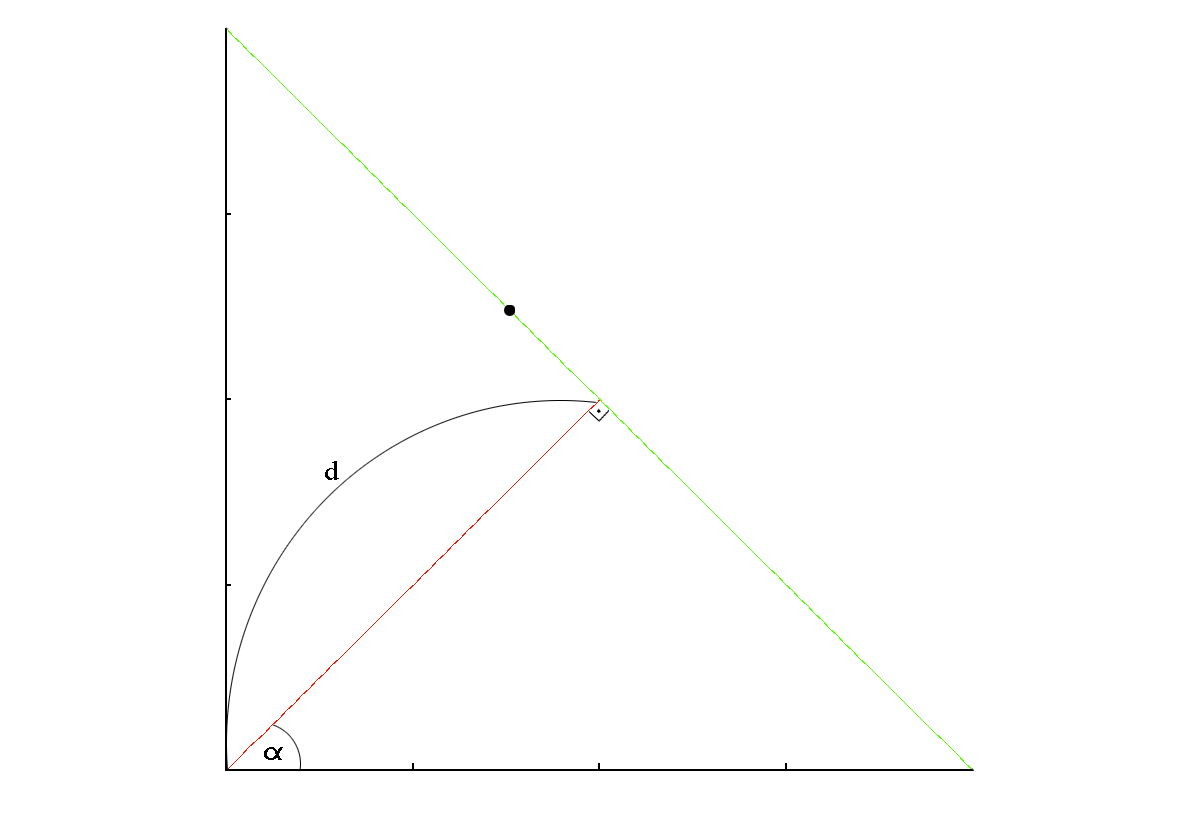
\includegraphics[scale=1.1]{img/Hough1.png}
  \caption{Anstatt Steigung und y-Achsenabschnitt werden als Parameter $\alpha$ und d genommen.}
\end{figure}
Wenn dies nun für alle vorhandene Kantenpunkte gemacht wird, werden im Parameterraum eine dementsprechende Anzahl von Kurven (oder Geraden) abgebildet, die einen exakten, oder ungefähren Schnittpunkt besitzen sollten. Die Parameter, die an diesem Punkt abgelesen werden, stellen die Parameter für unsere Kante im Bild durch die Kantenpunkte dar.\\\\
\begin{figure}[H]
  \centering
      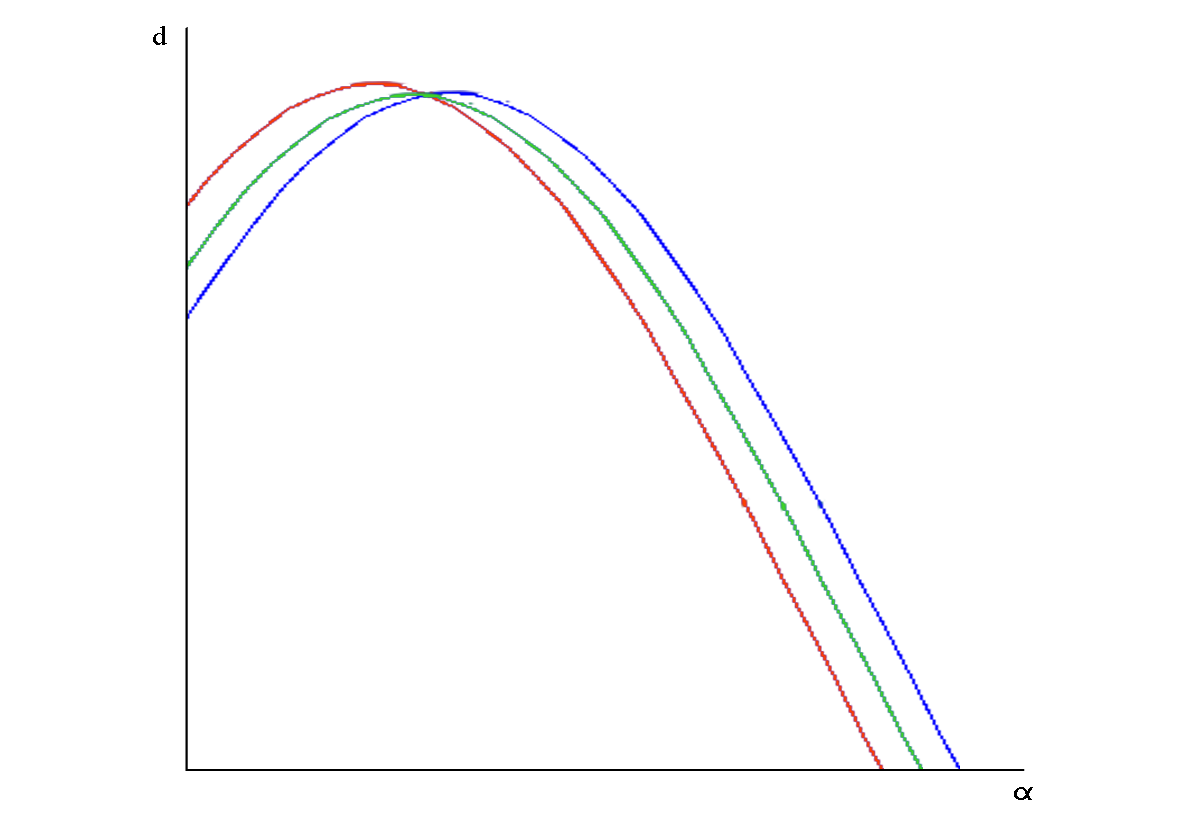
\includegraphics[scale=1.1]{img/Hough2.png}
  \caption{Überschneidung der Kurven im Parameterraum geben an, welche Parameter für die gesuchte Gerade zu nutzen sind.}
\end{figure}
Möchte man nun einen Kreis im Bild finden, werden von den Kantenpunkten alle möglichen Kreisgleichungen aufgestellt, dementsprechend als Parameter der Radius und der Mittelpunkt $(x,y)$ gewählt, womit wir einen dreidimensionalen Parameterraum haben.\\
Unter berücksichtigung eines Maximalwertes für den Radius tut man dies für alle Kantenpunkte, und anschließend lässt sich im Parameterraum wieder ein Schnittpunkt ablesen, an der sich die Parameter des gesuchten Kreises befinden.\\\\
\begin{figure}[H]
  \centering
      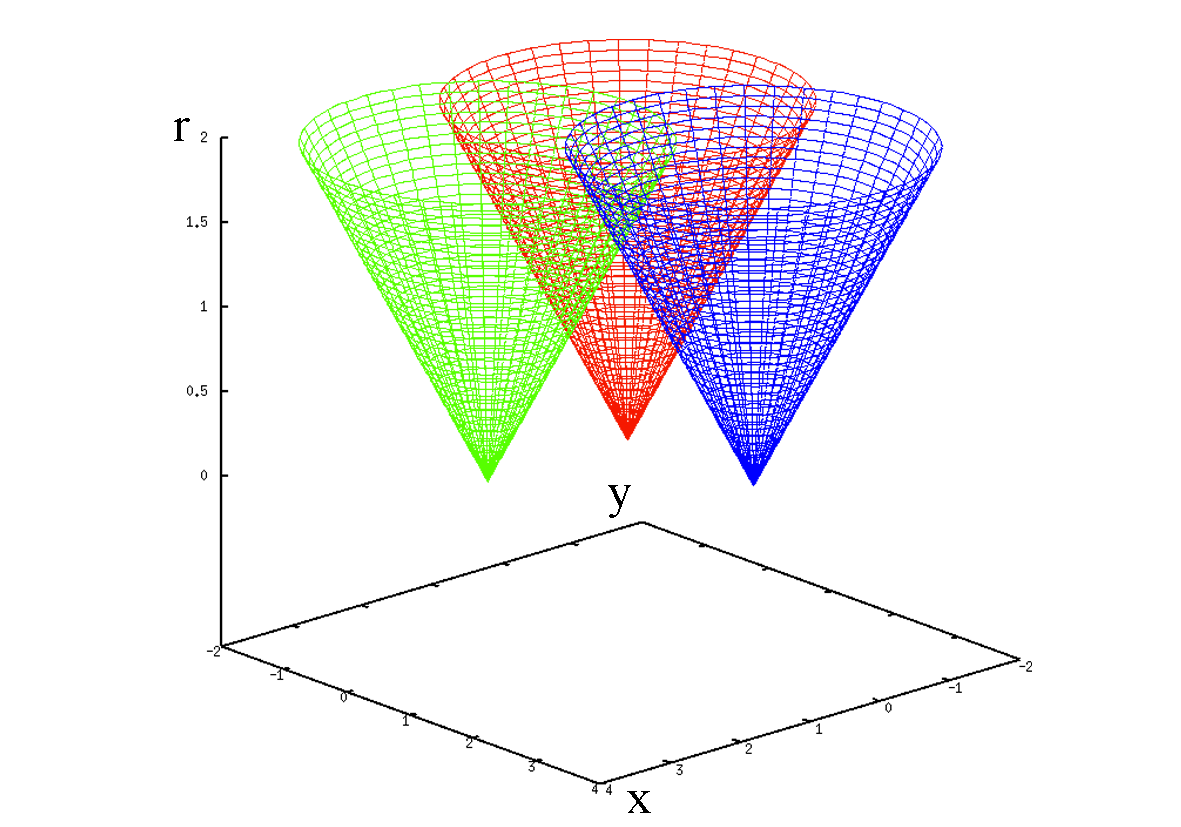
\includegraphics[scale=1.1]{img/Hough3.png}
  \caption{Es entstehen Kegeln, an denen sich wieder ein Schnittpunkt bildet.}
\end{figure}
Dieses kann man für beliebige Formen anwenden, die durch eine Parameterdarstellung definiert werden können, aber je mehr Parameter vorhanden sind, desto aufwändiger wird auch die Berechnung werden.

Dieses Verfahren sollte genutzt werden, um die genauen Ballpositionen im Tiefen- oder auch RGB-Bild zu bestimmen. Wenn möglich, sollte nach dem Filtern nach Regions of Interest im Tiefenbild auf diesen gefundenen Regionen die Hough-Transformation durchgeführt werden, um Kreise bzw. Bälle zu finden, oder auch Regionen ohne Bälle ausschließen zu können.\\
Genutzt haben wir die Implementation der Hough-Transformation in der OpenCV\cite{opencv}-Bibliothek. Hierbei wurde festgestellt, dass durch Einstellen der Parameter der Funktion die Kreiserkennung sehr fein bestimmt werden kann. Da, wie in Abbildungen \ref{rects-1} bis \ref{rects-4} zu sehen ist, die Bälle fast nie als saubere Kreise mit scharfen Kanten aufgenommen werden, war das Feintuning der Parameter unmöglich. Entweder wurde sehr grob eingestellt, so dass alle Bälle zwar erkannt wurden, dabei aber noch viel mehr False-Positives entstanden, oder es wurde so fein eingestellt, dass nur sehr sauber aufgenomme Bälle erkannt wurden. Bei letzterem wurden insgesamt aber viel zu wenige Bälle gefunden, so dass durch Einsetzen dieses Verfahren in unserem Fall kein Vorteil, sondern nur Nachteile entstanden.\\
Zudem wurde festgestellt, dass dieser Algorithmus viel Rechenleistung beansprucht und durch viel Kreisdetektion die ausgegebene Frame-Rate sank.

Die Überlegung war, dass durch eine Einbindung des Algorithmus als C-Code, z.B. mit Cython, dieser Leistungsverlust ausgeglichen werden könnte. Durch eine eigene Implementation hätte die Ballerkennung evtl. auch verbessert werden können, so dass nicht nach Kreisen gesucht wird, sondern nach Ellipsen (in bestimmter Ausrichtung). Da aber die ersten Versuche nicht sonderlich erfolgreich waren und der Aufwand nicht lohnenswert erschien, wurde dagegen entschieden. Durch geschicktes filtern nach unseren Regions of Interest konnten diese auch soweit verkleinert werden, dass eine zusätzliche Beschränkung dieser nicht notwendig wurde. Auch das Entfernen von False-Positives in den Regions of Interest wurde auf anderem Wege gelöst.

\subsubsection{Local Maxima}
Mit Local Maxima werden lokale Maxima, also positive extreme Datenpunkte in einer lokal begrenzten Umgebung, bezeichnet.\\
Anfangs hatten wir die Idee, über lokale Maxima die Bälle im Tiefenbild zu finden. Dies würde bedeuten, dass im Tiefenbild nach allen Datenpunktanhäufungen gesucht wird, die möglichst nahe der Kamera sind, dabei aber innerhalb eines gegebenen Radius bleiben. Diese sollen zusätzlich von Datenpunkten umgeben sein, die einen deutlichen Abstand nach hinten zu diesen Datenpunktanhäufungen besitzen.\\
Umgangssprachlich würden wir also alle Objekte bestimmter Größe suchen, die sich in einem bestimmten Abstand zu ihrem Hintergrund befinden. Damit ließe sich ein flexibler Abstand von Jongleur zu Kinect bewerkstelligen, es könnte damit sogar eine Ortsveränderung des Spielers während der Jonglage verarbeiten.

In unserem Projekt werden die Tiefendaten zumeist als Numpy-Arrays verarbeitet und von Filter zu Filter gereicht. So war hier die Idee, einen weiteren Filter zu erstellen, in dem im Numpy-Array nach lokalen Maxima bestimmter Größe gesucht wird, um eine Vorauswahl von Regions of Interest zu bekommen. In diesen sollten in weiteren Schritten False Positives ausgeschlossen werden, um am Ende nur Regionen mit Bällen zu erhalten, in denen mit z.B. der Hough-Transformation (zu diesem Zeitpunkt wollten wir diese noch nutzen) die Bälle extrahiert werden sollten.

Für das Finden von Maxima im Numpy-Array werden die Python Module Numpy\cite{numpy} und Scipy\cite{scipy} genutzt, welche eine große Auswahl an wissenschaftliche Funktionen besitzen. Besonders für mehrdimensionale Matrixberechnungen und weitere Bildverarbeitungsoperationen eignen sich diese Module sehr gut, da ihre Funktionen auf diese Probleme optimiert sind und meist schneller als eine eigene Implementierung sind.

Speziell mit den Funktionen {\tt scipy.ndimage.filters.maximum\_filter} und\\ {\tt scipy.ndimage.filters.minimum\_filter} wurden auf einem Tiefenbild die Maxima und Minima bis zu einem festgelegten Durchmesser gesucht. Durch Abziehen der Minima von den Maxima konnte auf dem daraus resultierenden Array mit einem Schwellwert, welcher den Abstand eines Maxima zu seiner Umgebung beschreibt, lokale Maxima bestimmter Größe gefunden werden.

Dieses Verfahren, welches bei Testbildern, welche rauscharm mit einem gleichmäßigen Hintergrund sind, auf dem deutlich hellere Punkte verteilt sind, funktioniert gut. In unserem Falle aber bestand das Problem, dass bei verschiedenen Einstellungen der Parameter entweder zu viele Maxima, wie beispielsweise jede sich hervorhebende Falte in der Bekleidung des Spielers gefunden wird, oder aber zu wenige, so dass sich nicht alle Bälle immer in den Regions of Interest befinden würden.\\
So haben wir uns entschieden, keinen flexiblen Abstand des Spielers zur Kinect zuzulassen, sondern diesen festzulegen. Anfangs als Nachteil empfunden, stellten wir aber fest, dass dies schnell akzeptiert werden konnte und den Spielspaß nicht mindert.

Unsere finale Umsetzung zum Finden von Regions of Interest wird in Abschnitt \ref{sec:roi} beschrieben.

\subsection{Ballerkennung}
{\color{red} FIXME ROLF Python Code mit Wurfparabel und Erklären usw}

Als erste Idee, um falsche Positionen auszuschließen, dachten wir an eine
Ballerkennung auf den RGB-Daten im Umfeld der Position. Naheliegend war die die
Implementierung einer Hough-Transformation, mit der wir auch begonnen haben.
Erste Testläufe auf den RGB-Daten der Kinect zeigten aber, dass je nach Wahl der
Parameter entweder die Bälle nicht erkannt, oder aber viel zu viele false-positives
erkannt wurden. Dies lag vor allem an den sehr verwischten Aufnahmen der Bälle
während des Fluges. Bei Betrachtung der Beispielaufnahmen (siehe oben) wird auch
deutlich, dass eine vermutete Position teilweise deutlich von der tatsächlichen
Position in den Bilddaten abwich. Somit konnten wir durch diesen Ansatz keinen Gewinn
ziehen, so dass wir uns auch durch die Abweichungen zwischen Ballposition in RGB- und
Tiefendaten dazu entschlossen, uns alleine auf eine Untersuchung der Tiefendaten zu
stützen.

Aber auch für die reine Berücksichtigung der Tiefendaten haben wir während des
Projektablaufes mehrere Problemquellen identifizieren können, die die verschiedenen
Ansätze unterschiedlich stark beeinflussen:

\begin{itemize}
 \item Die Hände sind auch in den möglichen Ballpositionen als Rechtecke enthalten.
 \item Die Bälle fliegen sehr nahe beieinander und teilweise überschneiden sich die Rechtecke zweier Bälle, so dass nur ein großes Rechteck zu sehen ist und als eine mögliche Ballposition untersucht wird.
 \item Ein Ball legt in einem Frame (1/30 Sekunde) unterschiedlich lange, teilweise sehr große Strecken zurück. (Pixelanzahl angeben?)
 \item Der Mindestabstand zur Kinect resultiert in einem kleinen Jongliermuster, wodurch die problematischen Faktoren verstärkt werden.
 \item In aufeinander folgenden Frames wird zum Teil eine Region in einigen der Frames nicht erkannt, in anderen schon.
\end{itemize}

Diese Problemquellen wirken sich unterschiedlich stark auf die Eignung der von
uns im folgenden betrachteten Ansätze aus. Prinzipiell lassen sich die Ansätze
in zwei Gruppen unterteilen: In die erste Gruppe, bei der von vorneherein von einer
festen Ballanzahl ausgegangen wird und die zweite Gruppe, bei der auch eine dynamisch wechselnde Ballanzahl erlaubt ist.

Bei den Ansätzen mit fester Ballanzahl wird in jedem Verarbeitungsschritt versucht,
zu jeder bereits existierenden Ballinstanz eine Position aus den erkannten Rechtecken
auszuwählen, welche als neue Position des Balls festgelegt wird. Da im Allgemeinen nie
zwei Bälle an der gleichen Position sein können, wird dieses Rechteck dann für die weiteren Ballinstanzen nicht mehr betrachtet, wir nennen die folgenden Ansätze daher
auch \textit{konsumierende Ansätze}. FIXME: das ist falsch, konsumierend $\neq$ feste Ballanzahl.

 \begin{enumerate}
 \item Die zwei sich am nächsten Punkte in zwei aufeinander folgenden Frames werden als der identische Ball aufgefasst. Nicht so zuverlässig, vor allem wegen schneller Ballbewegungen und nahe aneinander passierender Bälle. Schwierig auch, wenn ein erkannter Ball fehlt $\rightarrow$ Beachtung von ``springenden'' Bällen.
 \item Verbesserungsansatz: Die erwartete Ballposition wird mit der vorherigen Bewegung (linearer Bewegungsvektor) approximiert. Dies ist teilweise besser, aber trotzdem noch schwierig, die initiale Bewegung zu Erkennen. Hierbei verbleiben auch weiterhin Probleme mit Lücken in den Informationen.
 \item Weitere Verbesserung: Keinen linearen Bewegungsvektor nutzen, sondern die Flugbahn vorberechnen. Der lineare Bewegungsvektor wird als Tangente an der Steigung der Wurfparabel zu Grunde gelegt. (Verbesserung nochmal gut angucken, aber gefühlt hat das erstaunlich wenig unterschied gebracht)
 \end{enumerate}


Im Gegensatz dazu sind die folgenden nicht konsumierende Ansätze zu sehen, bei denen
wir auch eine variable Ballanzahl erlauben. FIXME: das ist falsch, siehe oben

\begin{enumerate}
	\item Wenn eine langsame Aufwärtsbewegung in aufeinander folgenden Frames erkannt wird: als Beginn eines Wurfes auffassen und an dieser Stelle einen Ball mit identischer Geschwindigkeit starten und dessen Flugbahn ab dort schrittweise simulieren. In jedem Schritt mit aktuell vorhandenen Bällen abgleichen und Wurfparameter anpassen. (hier schrittweise Bilder zeigen: Feuerwerk etc)
	\item Wie der Ansatz davor, allerdings wird die Parabel nicht approximiert, sondern	aus den letzten 3 Frames mit \lstinline{np.polyfit} berechnet.
\end{enumerate}

{\color{red} FIXME} Hier nochmal Codebeispiel zu den Ansätzen, die Wurfparabel zu berechnen.

In den ersten Versuchen, den Wurf zu modellieren, wurde die Idee von Kalman aufgegriffen und auf sehr einfache Weise versucht, diese umzusetzen. Dazu wurde erst einmal die Bewegung des Balls als eine Wurfparabel bestimmt, dessen mathematische Formel wie folgend ist:
\begin{align}
x& = v_{x}t \\
y& = v_{0_{y}t} - \frac{g}{2}t^{2}
\end{align}
Die Bewegung in der x-Achse, also der Horizontalen, ist eine Bewegung mit konstanter Geschwindigkeit $v$ über die Zeit $t$. In der Vertikalen y-Achse wirkt die Schwerkraft mit konstanter Geschwindigkeit $g=9,81 \frac{m}{s^{2}}$ nach unten auf den Ball ein. Hiermit lässt sich eine Position des Balls bei Zeitpunkt $t$ bestimmen, wenn Anfangsposition und Geschwindigkeiten in beide Richtungen bekannt sind. In unserem Fall kann eine Anfangsposition bestimmt werden, jedoch ist aus einem Frame allein die Geschwindigkeit nicht zu bestimmen. Werden mindestens zwei Frames genutzt, und in diesen Bälle gefunden, die einander zugeordnet werden, kann hieraus eine Anfangsposition und zusätzlich eine Richtung sowie Geschwindigkeit gewonnen werden. Da nun anstatt der Geschwindigkeit in horizontaler und vertikaler Richtung nur eine allgemeine Geschwindigkeit des Balles, aber zusätzlich eine Richtung extrahiert werden konnte, werden folgende Formeln für den Ballwurf genutzt:
\begin{align}
x(t)& = v_{0}t\cos\beta \\
y(t)& = v_{0}t\sin\beta - \frac{g}{2}t^{2}
\end{align}
Mit $v_{0}$, der Geschwindigkeit des Balles und $\beta$, dem Winkel, in dem der Ball schräg nach oben geworfen wird, kann nun intern der Wurf modelliert werden.

Ein Beispiel einer einfachen Implementierung dessen mit zwei vorgegebenen Ballpositionen:

\begin{lstlisting}[language=Python]
class SimpleKalmanFilter(object):

    def trajectory(self, (y1, x1), (y2, x2), t):
        b = np.degrees(np.arctan((y2-y1)/(x2-x1)))  # Winkel, in dem hochgeworfen wird
        v = np.sqrt((x1 + x2)**2 + (y1 + y2)**2)    # Geschwindigkeit des Balls
        x = v * t * np.degrees(np.cos(b))
        y = v * t * np.degrees(np.sin(b) - (9.81/2) * t**2)
        return (y,x)

    def filter(self, rgb, depth, balls, args = {}):
        p1 = (480, 0)
        p2 = (470, 10)
        points = []

        for t in xrange(1,10):
            point = self.trajectory(p1, p2, t)
            points.append(point)

        return points
\end{lstlisting}
Hierbei wird durch Aufruf von {\tt SimpleKalmanFilter.filter} für zwei aufeinanderfolgenden Ballpositionen in einer Schleife für 10 Zeiteinheiten eine voraussichtliche Wurfbahn berechnet und zurückgegeben.

Leider schlug dieser Ansatz fehl, 

{\color{red}FIXME Warum dies nicht klappt, die nächsten Ansätze und wie es gelöst wurde}

\section{Herausforderungen}

{\color{red}Probleme aus den Ansätzen noch mal aufgreifen. Noch irgendwas abstrakteres dazu schreiben? Vielleicht dass wir uns nicht doll genug getracked haben dier Projektzeit über? Vielleicht nochmal die Reihenfolge sortieren.}

Während dieses Projektes wurden viele Ideen eingebracht, einige sofort implementiert, andere nach mehreren Versuchen nutzbar gemacht. Aber einige Ansätze konnten auch nach wiederholten Versuchen nicht ausreichend umgesetzt werden, oder schienen nach mehrmaligem Testen nicht den erhofften Fortschritt hineinzubringen, weswegen sie letzten Endes nicht in der Software genutzt werden.

Einige dieser Ansätze, die uns Schwierigkeiten bereitet haben, werden hier kurz vorgestellt, das Problem der Idee aufgezeigt, und wie wir sie letzten Endes doch implementiert haben - oder warum sie es nicht in die Software schafften.\\
Leider machten wir während des Projektes wenige Aufzeichnungen über unsere Arbeit, sondern schrieben wild drauf los, und was nicht funktionierte, wurde überschrieben. Deswegen ein Reminder an uns: Mehr Kommentieren und Fortschritt sowie Missglücktes notieren!


\subsection{Technische Herausforderungen}

Im Laufe des gesamten Projektes haben wir drei Projektteilnehmer verteilt auf drei
Betriebssystemen gearbeitet (Mac OS, Windows, Ubuntu). Da wir gerade dank
unseres flexiblen Filterkonzeptes gut arbeitsteilig arbeiten konnten, haben wir
nicht von Anfang an auf die Integrierbarkeit unserer Komponenten geachtet.

Der funktionierende Temporalfilter (siehe \ref{sec:temporal}) etwa wurde mit Hilfe
der Bildverarbeitungsbibliothek VIGRA\cite{vigra} implementiert. Die
Python-Bindings hierfür liegen nicht auf allen Systemen in gleich guter Verfügbarkeit
vor (zumindest war es uns auf Mac OS nicht möglich, diese ohne Mac Ports zum Laufen
zu bekommen, da die per \lstinline{pip install} verfügbare Version veraltet ist und
scheinbar nicht mehr gepflegt wird. (FIXME source)

Da der Temporalfilter zum einen der einzige Filter mit VIGRA Abhängigkeit war, und
der Filter zudem nicht die gewünschten Vorteile geliefert hat, die wir uns erhofft
hatten, haben wir diesen Filter nicht weiter in der Entwicklung betrachtet und so
auch die zusätzliche Dependency eingespart.

\subsection{Selbstorganisation und Arbeitsweise}

In unserer Arbeitsweise ist uns deutlich geworden, dass die Arbeit an praktischen
Projekten einen großen Lerneffekt hat und auch die zahlreichen Fehlversuche mit
wiederkehrenden frustrierenden Ergebnissen dazugehören, um schließlich zu einer
funktionierenden und robusten Implementierung zu gelangen. Um bei ähnlichen
Projekten in Zukunft schneller zu einem Ergebnis zu kommen, wird es aber nötig
sein, dass wir uns von Anfang an selbst klarere Ziele stecken und den Fortschritt
besser zu verfolgen um ihn auch sicher stellen zu können. %FIXME: das klingt etwas negativer. Vielleicht also nicht im Fazit nennen sondern davor noch einen Abschnitt über unsere Arbeitsweise während des Projekts?





\section{Bewertung des Endergebnisses}

{\color{red} FIXME ROLF ausformulieren und mit Kinect austesten!}

Vergleichen mit Zielsetzung

Robustheit.

  - Position des Jongleurs (Bildzentrum VS Bildrand. Abstand zur Kinect)

  - Objekte am Bildrand (bewegte vs nicht bewegte)

  - Ungleichmäßiges Jongliermuster

  - Variation der Bälleanzahl

Effizienz. Speedup-Möglichkeiten?

Anwendungsrelevanz.

\section{Anwendungsmöglichkeiten}

Die Grundidee des Projektes bestand in der Erstellung eines Systems zum Erkennen und
Verfolgen von Jonglierbällen in Echtzeit. Als Ziel hinter dieser Idee ist die
Möglichkeit gesehen, mit den gewonnenen Informationen verschiedene Anwendungen zu
ermöglichen. Das Projekt kann im aktuellen Zustand als Grundlage genommen werden
für einfache Programme und Spiele.

\subsection{Idee: Ein interaktiver Jongliertrainer}

Als denkbare Anwendung auf Basis der von uns erstellten Vorverarbeitung ist ein
interaktiver Jongliertrainer zu nennen. Ein solches Programm würde automatisch die
Qualität und Güte eines Jongliermusters erkennen und so über die Zeit den Fortschritt
der jonglierenden Person aufzeichnen.

Hierzu sind mehrere Grundaufgaben zu lösen, dessen Implementierung wir teilweise
bereits in unser Projekt aufgenommen haben.

\subsubsection{Objekte zählen}

Mit den erkannten momentan fliegenden Objekten haben wir als erste Anwendung einen
einfachen Zähler geschrieben, der die tatsächliche Anzahl der im Muster befindlichen Objekte zu bestimmen versucht.

Denke wäre eine Verfolgung der Objekte über einen längeren Zeitraum, um auch
unabhängig voneinander erkannte Objekte in ihrer Identität zu bestimmen. Tatsächlich
ist ein deutlich simplerer Ansatz aber bereits sehr effektiv, indem über eine
längere Anzahl Frames geschaut wird, wie viele Objekte in der Luft sind. Es wird der
Durchschnitt dieser Werte gebildet und aufgerundet. Auf diesen Wert wird dann noch
$1$ addiert, um zur tatsächlichen Anzahl zu gelangen. Dies ist der Tatsache
geschuldet, dass beim normalen Jongliermuster zu jeder Zeit mindestens ein Objekt in der Hand ruht, es kann also davon ausgegangen werden, dass maximal $n - 1$ Objekte
gleichzeitig in der Luft sind.

Ausprobieren auf echten Daten hat ergeben, dass beim Mitteln über $15$ Frames
ein zuverlässiges Bestimmen des tatsächlichen Wertes möglich ist.

\begin{lstlisting}[language=Python]
class BallCounter(object):
    """Determine the actual number of objects in the juggling pattern."""
    def __init__(self):
        self.count = None
        self.last = []
        self.length = 15 # how many frames to analyse

    def update(self, balls):
        self.last.append(len(balls))
        if len(self.last) > self.length:
            self.count = sum(self.last[::-1][:self.length]) / (self.length*1.0)
            self.count = int(math.ceil(self.count)) + 1
\end{lstlisting}


\begin{figure}[H]
    \centering
    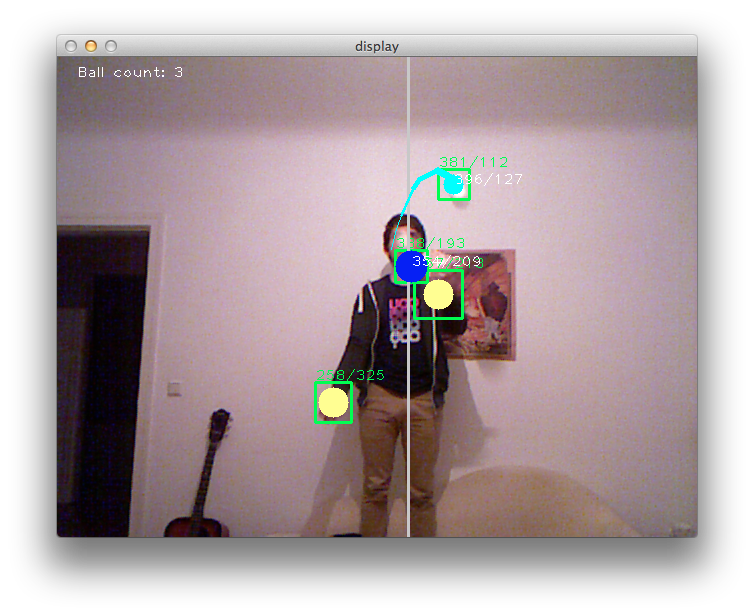
\includegraphics[scale=0.5]{img/ballcount-1.png}
    \vspace{-0.5cm}
    \caption{FIXME}
    \label{ballcount-1}
\end{figure}

\begin{figure}[H]
    \centering
    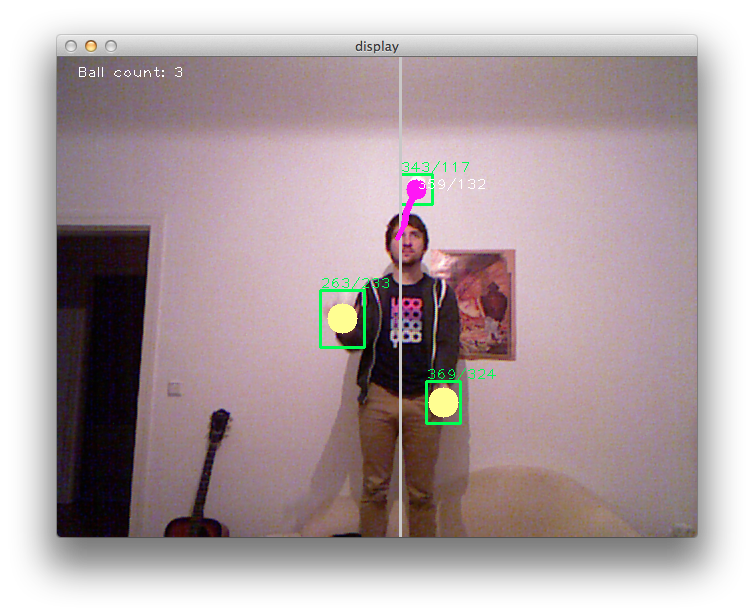
\includegraphics[scale=0.5]{img/ballcount-2.png}
    \vspace{-0.5cm}
    \caption{FIXME}
    \label{ballcount-2}
\end{figure}


\subsubsection{Würfe zählen}

Eine weitere Möglichkeit ist das Zählen von aufeinander folgenden Würfen. Dies ist
bereits ein Schritt in die Richtung eines Jongliertrainers, der den Fortschritt eines
Jongleurs über eine gewisse Zeit aufzeichnet und misst.

Als Herausforderung bei der Implementierung ist zuerst die Tatsache zu nennen, dass
es in den von uns bisher betrachteten Testdaten öfter vorkommt, dass ein Ball in
einem Frame nicht erkannt wird, da der Sensor hier keine zuverlässigen Informationen
liefert. Im bisherigen Modell wird dadurch das Ballobjekt verworfen und erst im
darauf folgenden Frame ein neues initialisiert. Das Zählen von Würfen stimmt
also nicht mit dem Zählen von Ball-Initialisierungen überein.

Denkbare Lösungsansätze wären hier, die zwei (oder mehr) Teile einer unterbrochenen
Wurfparabel zu erkennen und den Zwischenschritt zu interpolieren, um die gesamte
Wurfbahn als einen einzelnen Wurf aufzufassen.

Wird die zeitliche Verteilung der Würfe aufgezeichnet, lässt sich auch analysieren,
wie gleichmäßig der Jonglier-Rhythmus ist. Auch dies ist ein wichtiger Faktor

\subsubsection{Wurfhöhen messen}

Ein gutes Jongliermuster zeichnet sich durch seiner Gleichmäßigkeit aus. Dies trifft
sowohl auf

\subsection{Idee: Siteswaps erkennen}

Bisher haben wir immer über die Grundmuster beim Jonglieren gesprochen, bei denen
Bälle im gleichmäßigen Rhythmus auf gleicher Höhe immer die gleichen Wurfbahnen
durchlaufen. Tatsächlich existieren komplexere Jongliermuster, die gewissen Regeln
folgen müssen, damit in einem gleichmäßigen Rhythmus jongliert werden kann, die Bälle
verschieden hohe Flugbahnen verfolgen können, und dabei nie zwei Objekte zur gleichen
Zeit in der Hand landen.

Eine Notation zur Aufzeichnung solche Muster ist die \textit{Siteswap-Notation}, ein
entsprechend jongliertes Muster wird verkürzt als \textit{Siteswap} bezeichnet.
Vereinfacht gesagt sind Siteswaps für das Jonglieren so etwas wie Noten für Musiker.
Die Notation besteht hierbei grundlegend aus Zahlenreihen, wobei jede Stelle der
Reihe einem Wurf entspricht, der Wert an der Stelle bestimmt die Höhe des Wurfes.

Der Siteswap \textit{531} etwa besteht aus drei Würfen. Die \textit{5} entspricht
einem Wurf der Höhe von einer regulären 5-Ball-Jonglage, die \textit{3} entsprechend
der Höhe einer 3-Ball-Jonglage. Da laut offizieller Regelung (FIXME source) eine
Jonglage erst dann als Jonglieren zählt, wenn mehr Objekte als Hände beteiligt sind,
haben die Werte Zwei, Eins und Null eine Sonderbedeutung. Die Null im Siteswap
bezeichnet eine leere Position zu diesem Takt, die Eins ist ein Übergeben des
Objektes von einer in die andere Hand und die Zwei bedeutet ein Festhalten des Balles
während einer Zählzeit.

Die konkreten Wurfhöhen sind hierbei nicht von der Zahlenvorschrift festegelegt, sie
bezeichnen lediglich relative Höhenabstände zueinander.

Siteswaps sind zudem periodisch zu verstehen, können also fortlaufend jongliert
werden. Der oben betrachtete Siteswap \textit{531} ist also gleichbedeutend mit
\textit{531531531$\dots$}.

Tatsächlich tragen die Zahlen bereits viel Information, die nicht erst beim
Jonglieren sichtbar wird. So ist ein Siteswap immer nur mit einer bestimmten
Objektanzahl möglich, die dem Durchschnitt der einzelnen Wurfwerte entspricht.
Teilt man also die Quersumme von \textit{531} ($= 9$) durch die Anzahl der Würfe
($3$), sieht man, dass dies tatsächlich ein 3-Ball-Muster ist. Hierbei sind nur
ganzzahlige Ergebnisse möglich. \textit{541} etwa wäre kein valider Siteswap und ist
nicht jonglierbar.

Wie an Hand dieser kurzen Einführung bereits deutlich wird, bieten Siteswaps sich gut
zur automatischen Analyse an. Möglich und denkbar ist also eine Anwendung, die an
Hand der von unserem System gelieferten Daten automatisch Siteswaps erkennt.

Hierbei wären folgende grundlegenden Schritte notwendig.

\begin{enumerate}
\item Würfe mit ihren absoluten Wurfhöhen aufzeichnen
\item Würfe nach Abwurfzeit sortieren
\item Relative Wurfhöhen bestimmen
\item Bei möglichen Mehrdeutigkeiten das Wissen aus der Siteswap Theorie nutzen
\end{enumerate}

Mit Hilfe dieser Erkennung ist es denkbar, dem Akteur vor der Kinect Aufgaben an Hand
von Jongliermustern zu geben, die erfolgreich jongliert werden müssen. Ein Muster
kann animiert vorjongliert werden, der Akteur muss hierbei nicht einmal mit der
Zahlentheorie konfrontiert werden. So ist ein einfaches Level-basiertes System
denkbar, das einen Jonglieranfänger vom Grundmuster zu komplexeren Mustern und
sogar mehr als drei Jonglierobjekten führt.

\section{Fazit}

Im Laufe des Projektes haben wir uns intensiv mit der Echtzeitverarbeitung von
Tiefendaten auseinander gesetzt und sind über viele nicht funktionierende
Ansätze zu einem Ergebnis gekommen, das robust und mit flexibler Anzahl von
Objekten das Muster eines Jongleurs erfasst. Unsere für die erfolgreiche
Implementierung getroffenen Annahmen über den Aufbau der Kinect und die Position des
Jongleurs im Raum sind nicht all zu einschränkend, so dass einer tatsächlichen
Anwendung der entwickelten Software nichts im Wege steht.

Die Software kann als Grundlage verwendet werden für weitere Anwendungen mit
der Kinect und Jonglierbewegungen. Dies haben wir beispielhaft am Anwendungsfall
des Zählens von Jonglierbällen gezeigt und weitere mögliche Entwicklungen
vorgeschlagen und die nötigen Schritt umrissen.

Als Endergebnis des Projektes gelangen wir erfolgreich zu einer quelloffenen und flexibel
erweiterbaren Software, die robust unsere selbst gestellte Aufgabe löst. Zudem haben
bei der Arbeit mit den verwendeten Libraries viel gelernt und dem
\lstinline{libfreenect} in der Open Source Community bei der Verbesserung der
Code Basis helfen können.




\newpage



\newpage
\phantomsection
\addcontentsline{toc}{section}{Quellen}
\renewcommand{\refname}{Quellen}
\bibliographystyle{plain}
\begin{thebibliography}{99}

{\color{red}
\bibitem{FIXME}
FIXME Bibliothek evtl. etwas sortieren oder so}

%\cite{hacking}
\bibitem{hacking}
Jeff Kramer, Nicolas Burrus, Florian Echtler, Daniel Herrera C., Matt Parker\\
{\em Hacking the Kinect}\\
ISBN 978-1-4302-3867-6\\
Springer Science+Business Media New York, 2012.

\bibitem{kober}
Jens Kober$^{1,2}$, Matthew Glisson$^{2}$, and Michael Mistry$^{2,3}$,\\
{\em Playing Catch and Juggling with a Humanoid Robot}.\\
$^{2}$ Disney Research Pittsburgh, USA\\
$^{1}$ Bielefeld University, Germany,\\
$^{3}$ University of Birmingham, UK.

\bibitem{disneyresearch}
Jens Kober$^{1,2}$, Matthew Glisson$^{2}$, and Michael Mistry$^{2,3}$,\\
Disney Research Project Web Page\\
{\em Playing Catch and Juggling with a Humanoid Robot}.\\
$^{2}$ Disney Research Pittsburgh, USA\\
$^{1}$ Bielefeld University, Germany,\\
$^{3}$ University of Birmingham, UK\\
\url{http://www.disneyresearch.com/project/juggling_robot} (accessed on 2014-06-22).

\bibitem{openkinect}
{\em OpenKinect project}\\
\url{http://openkinect.org/wiki/Main_Page} (accessed on 2014-06-12).

\bibitem{libfreenect}
{\em libfreenect GitHub repository}\\
\url{https://github.com/OpenKinect/libfreenect} (accessed on 2014-06-12).

\bibitem{3dpuppetry}
Robert T. Held$^{1}$, Ankit Gupta$^{2}$, Brian Curless$^{2}$, Maneesh Agrawala$^{1}$\\
{\em 3D Puppetry: A Kinect-based Interface for 3D Animation}\\
$^{1}$ University of California, Berkeley,\\
$^{2}$ University of Washington,\\
Cambridge, Massachusetts, USA, 2012.

\bibitem{kinectavatar}
Yan Cui$^{1}$, Will Chang, Tobias Nöll$^{1}$, Didier Stricker$^{1}$\\
{\em KinectAvatar: Fully Automatic Body Capture Using a Single Kinect}\\
$^{1}$ Augmented Vision, DFKI,\\
German Research Center for Artificial Intelligence.

\bibitem{rgbzvideos}
Christian Richardt$^{1,2}$, Carsten Stoll$^{1}$, Neil A. Dodgson$^{2}$, Hans-Peter Seidel$^{1}$, Christian Theobalt$^{1}$\\
{\em Coherent Spatiotemporal Filtering, Upsampling and Rendering of RGBZ Videos}\\
$^{1}$ MPI Informatik,\\
$^{1}$ University of Cambridge,\\
EUROGRAPHICS Volume 31, Number 2, 2012.

\bibitem{vigra}
Ullrich Köthe und viele weitere Mitwirkende\\
{\em The VIGRA Computer Vision Library Version 1.10.0}\\
\url{http://ukoethe.github.io/vigra/} (accessed on 2014-06-24).

\bibitem{hough}
Richard O. Duda, Peter E. Hart,\\
{\em Use of the Hough Transformation to detect lines and curves in pictures}\\
Technical Note 36, Artificial Intelligence Center, April 1971,\\
Published in the  Comm. ACM, Vol 15, No. 1 (11-15), January 1972.\\
\url{http://www.ai.sri.com/pubs/files/tn036-duda71.pdf} (accessed on 2014-06-25).

\bibitem{opencv}
OpenCV (Open Source Computer Vision)\\
\url{http://opencv.org/} (accessed on 2014-06-25).

\bibitem{kalman}
Rudolf E. Kálmán\\
{\em A New Approach to Linear Filtering and Prediction Problems}\\
Transaction of the ASME, Journal of Basic Engineering, 35-45,\\
Research Institute for Advanced Study, Baltimore, Md., 1960.\\
\url{http://www.cs.unc.edu/~welch/kalman/media/pdf/Kalman1960.pdf} (accessed on 2014-06-26).

\bibitem{waas}
Federal Aviation Administration\\
Frequently Asked Questions - WAAS\\
\url{http://www.faa.gov/about/office_org/headquarters_offices/ato/service_units/techops/navservices/gnss/faq/waas/} (accessed on 2014-06-26).

\bibitem{egnos}
European Space Agency\\
What is EGNOS?
\url{http://www.esa.int/Our_Activities/Navigation/The_present_-_EGNOS/What_is_EGNOS} (accessed on 2014-06-26).

\bibitem{numpy}
Numpy\\
\url{http://www.numpy.org/} (accessed on 2014-06-28).

\bibitem{scipy}
Scipy\\
\url{http://www.scipy.org/} (accessed on 2014-06-28).

\end{thebibliography}

\end{document}
